\section{伊辛模型的Bethe解}
\subsection{数图的熵}
Bethe 方法采用树图的计数方式：在无环图 （树） 上可以严格推导并精确成立，而在一般含环格点图上仅作为近似.以下只考虑无环树图情形，先推导数图的熵.

记与第\(i\)个格点相邻的格点有\(d_i\)个（度为\(d_i-1\)），概率用\(P\)表示，任选一个根节点\(r\)，则树上每个节点 \(k\neq r\) 有唯一父节点\(\vb{\pi}(k)\).格点状态用\(\vb{\sigma}\)表示，对定义在树图上的任意联合分布 \(\{\vb{\sigma}\}\)，利用树的无环结构，可以将联合分布严格分解为相邻两点联合概率与单点概率的乘积形式
\begin{equation*}
	P\left(\{\vb{\sigma}\}\right) = P\left(\vb{\sigma}_r\right)\prod_{\substack{i\neq r}}P\left(\vb{\sigma}_i\big|\vb{\sigma}_{\vb{\pi}(i)}\right) = P\left(\vb{\sigma}_r\right)\prod_{\substack{i\neq r}}\frac{P\left(\vb{\sigma}_i,\vb{\sigma}_{\vb{\pi}(i)}\right)}{P\left(\vb{\sigma}_{\vb{\pi}(i)}\right)} = \frac{\prod_{(ij)}P\left(\vb{\sigma}_i,\vb{\sigma}_j\right)}{\prod_{i}\left(P\left(\vb{\sigma}_i\right)\right)^{d_i-1}}
\end{equation*}
其中 \(P\left(\vb{\sigma}_i\right)\) 是节点\(i\)状态为\(\vb{\sigma}_i\)的概率，\(P\left(\vb{\sigma}_i,\vb{\sigma}_j\right)\) 是邻近节点\(i,j\)状态为\(\vb{\sigma}_i,\vb{\sigma}_j\) 的概率
\begin{equation*}
	\sum_{\vb{\sigma}_i}P\left(\vb{\sigma}_i\right) = \sum_{\vb{\sigma}_i,\vb{\sigma}_j}P\left(\vb{\sigma}_i,\vb{\sigma}_j\right) = 1, \quad
	P\left(\vb{\sigma}_i,\vb{\sigma}_j\right) = P\left(\vb{\sigma}_j,\vb{\sigma}_i\right), \quad
	\sum_{\vb{\sigma}_j}P\left(\vb{\sigma}_i,\vb{\sigma}_j\right) = P\left(\vb{\sigma}_i\right)
\end{equation*}

不难证明自洽性
\begin{equation*}
	\sum_{\{\vb{\sigma}\}}P\left(\{\vb{\sigma}\}\right) = 1
\end{equation*}

则图的熵为
\begin{equation*}
	S/k = -\sum_{\{\vb{\sigma}\}}P\left(\{\vb{\sigma}\}\right)\ln P\left(\{\vb{\sigma}\}\right) = -\sum_{(ij)}\sum_{\vb{\sigma}_i,\vb{\sigma}_j}P\left(\vb{\sigma}_i,\vb{\sigma}_j\right)\ln P\left(\vb{\sigma}_i,\vb{\sigma}_j\right) + (q - 1)\sum_{i}\sum_{\vb{\sigma}_i}P\left(\vb{\sigma}_i\right)\ln P\left(\vb{\sigma}_i\right)
\end{equation*}

\subsection{Bethe图上的严格解}
\subsubsection{配分函数解法}

\begin{figure}[htbp]
	\centering
	\begin{subfigure}[b]{0.23\textwidth}
		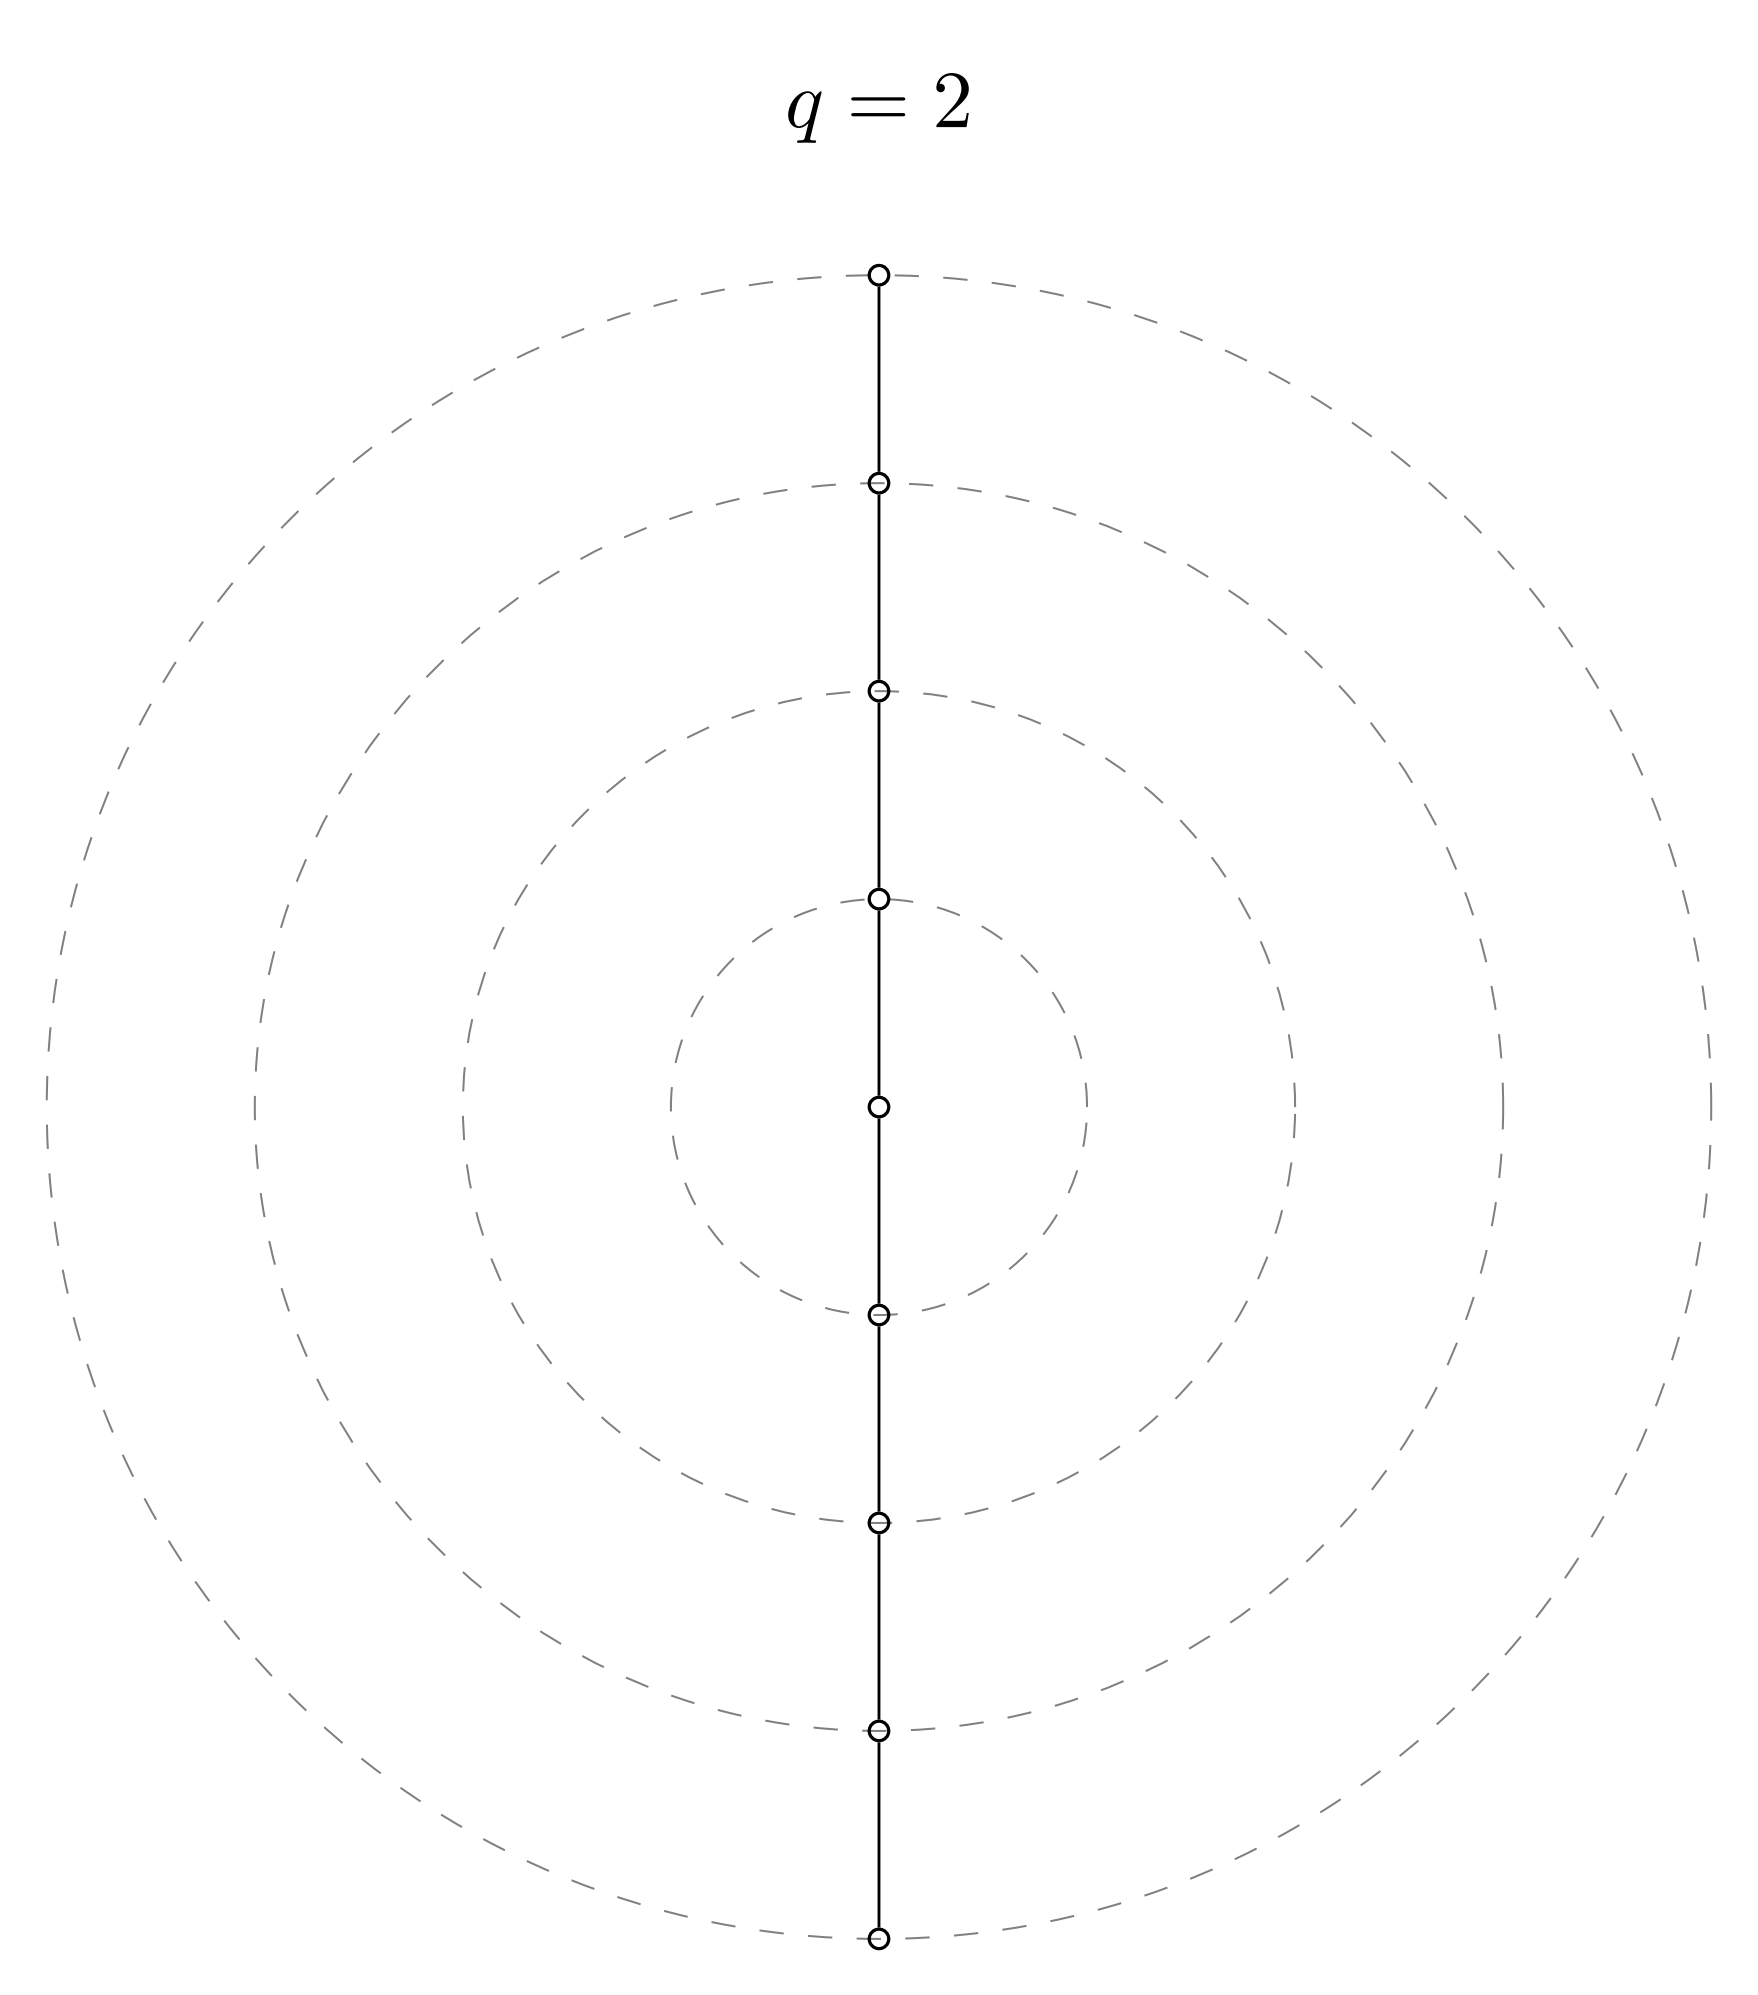
\includegraphics[width=\textwidth]{ising_model_fig/bethe_infinite_tree_level_1.png}
	\end{subfigure}
	\hfill
	\begin{subfigure}[b]{0.23\textwidth}
		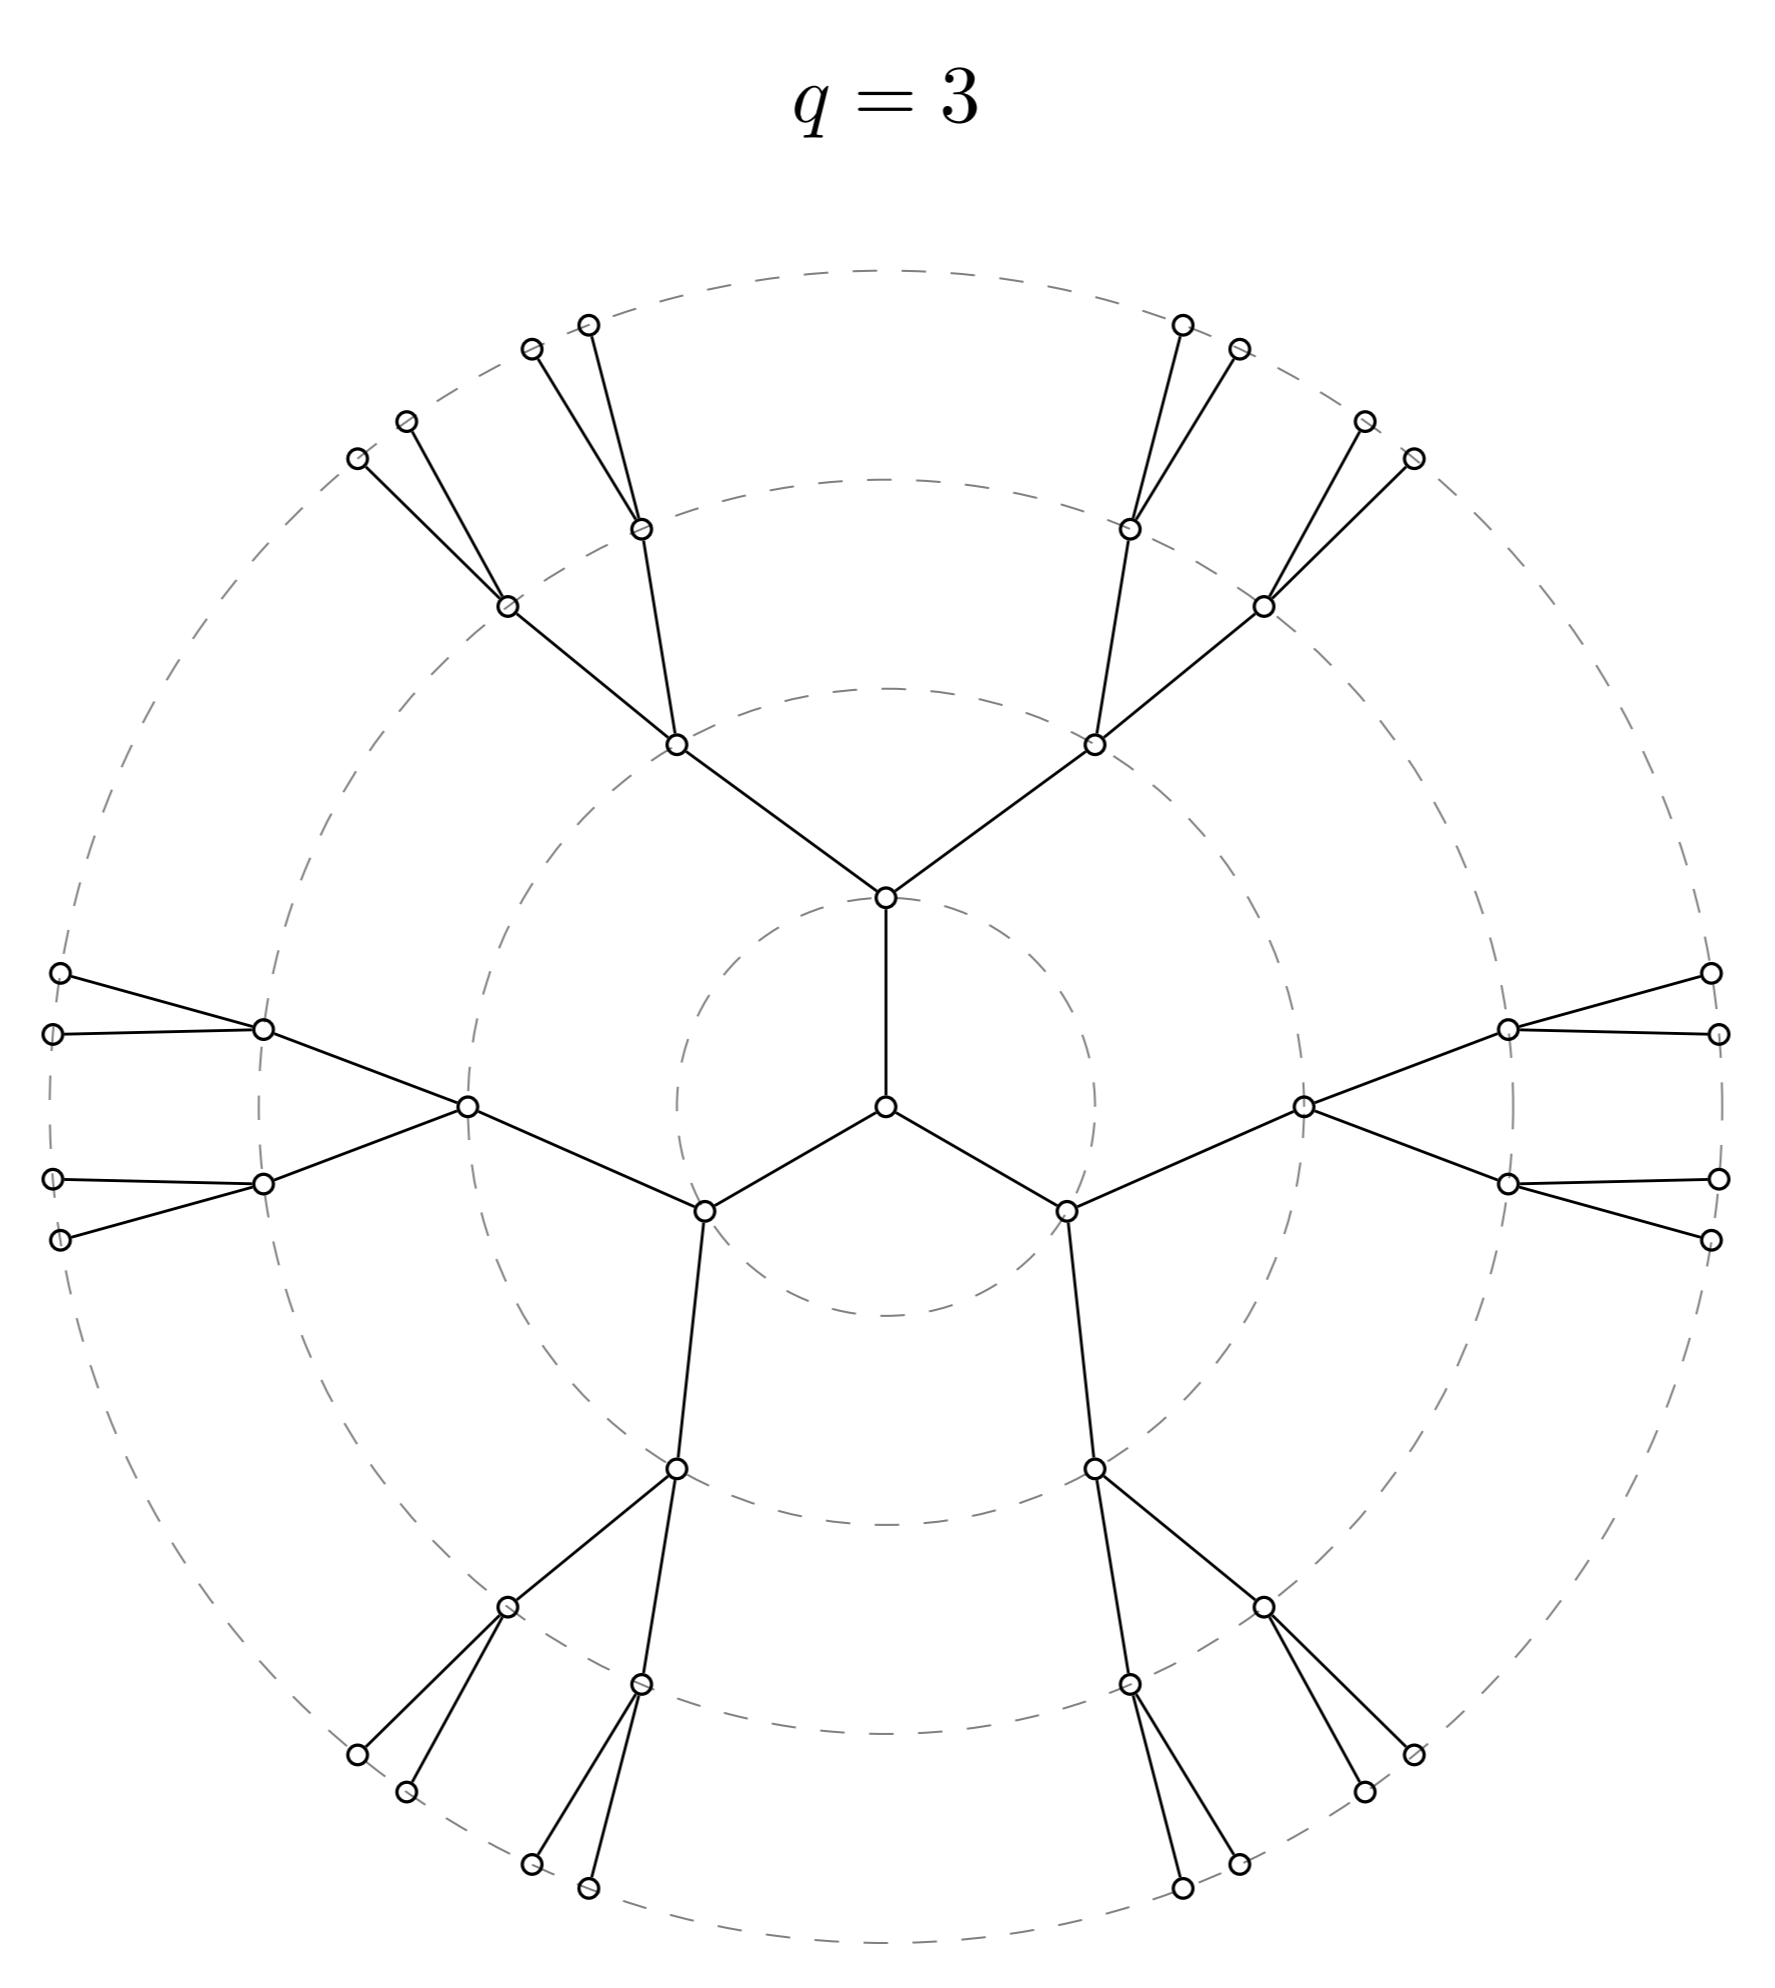
\includegraphics[width=\textwidth]{ising_model_fig/bethe_infinite_tree_level_2.png}
	\end{subfigure}
	\hfill
	\begin{subfigure}[b]{0.23\textwidth}
		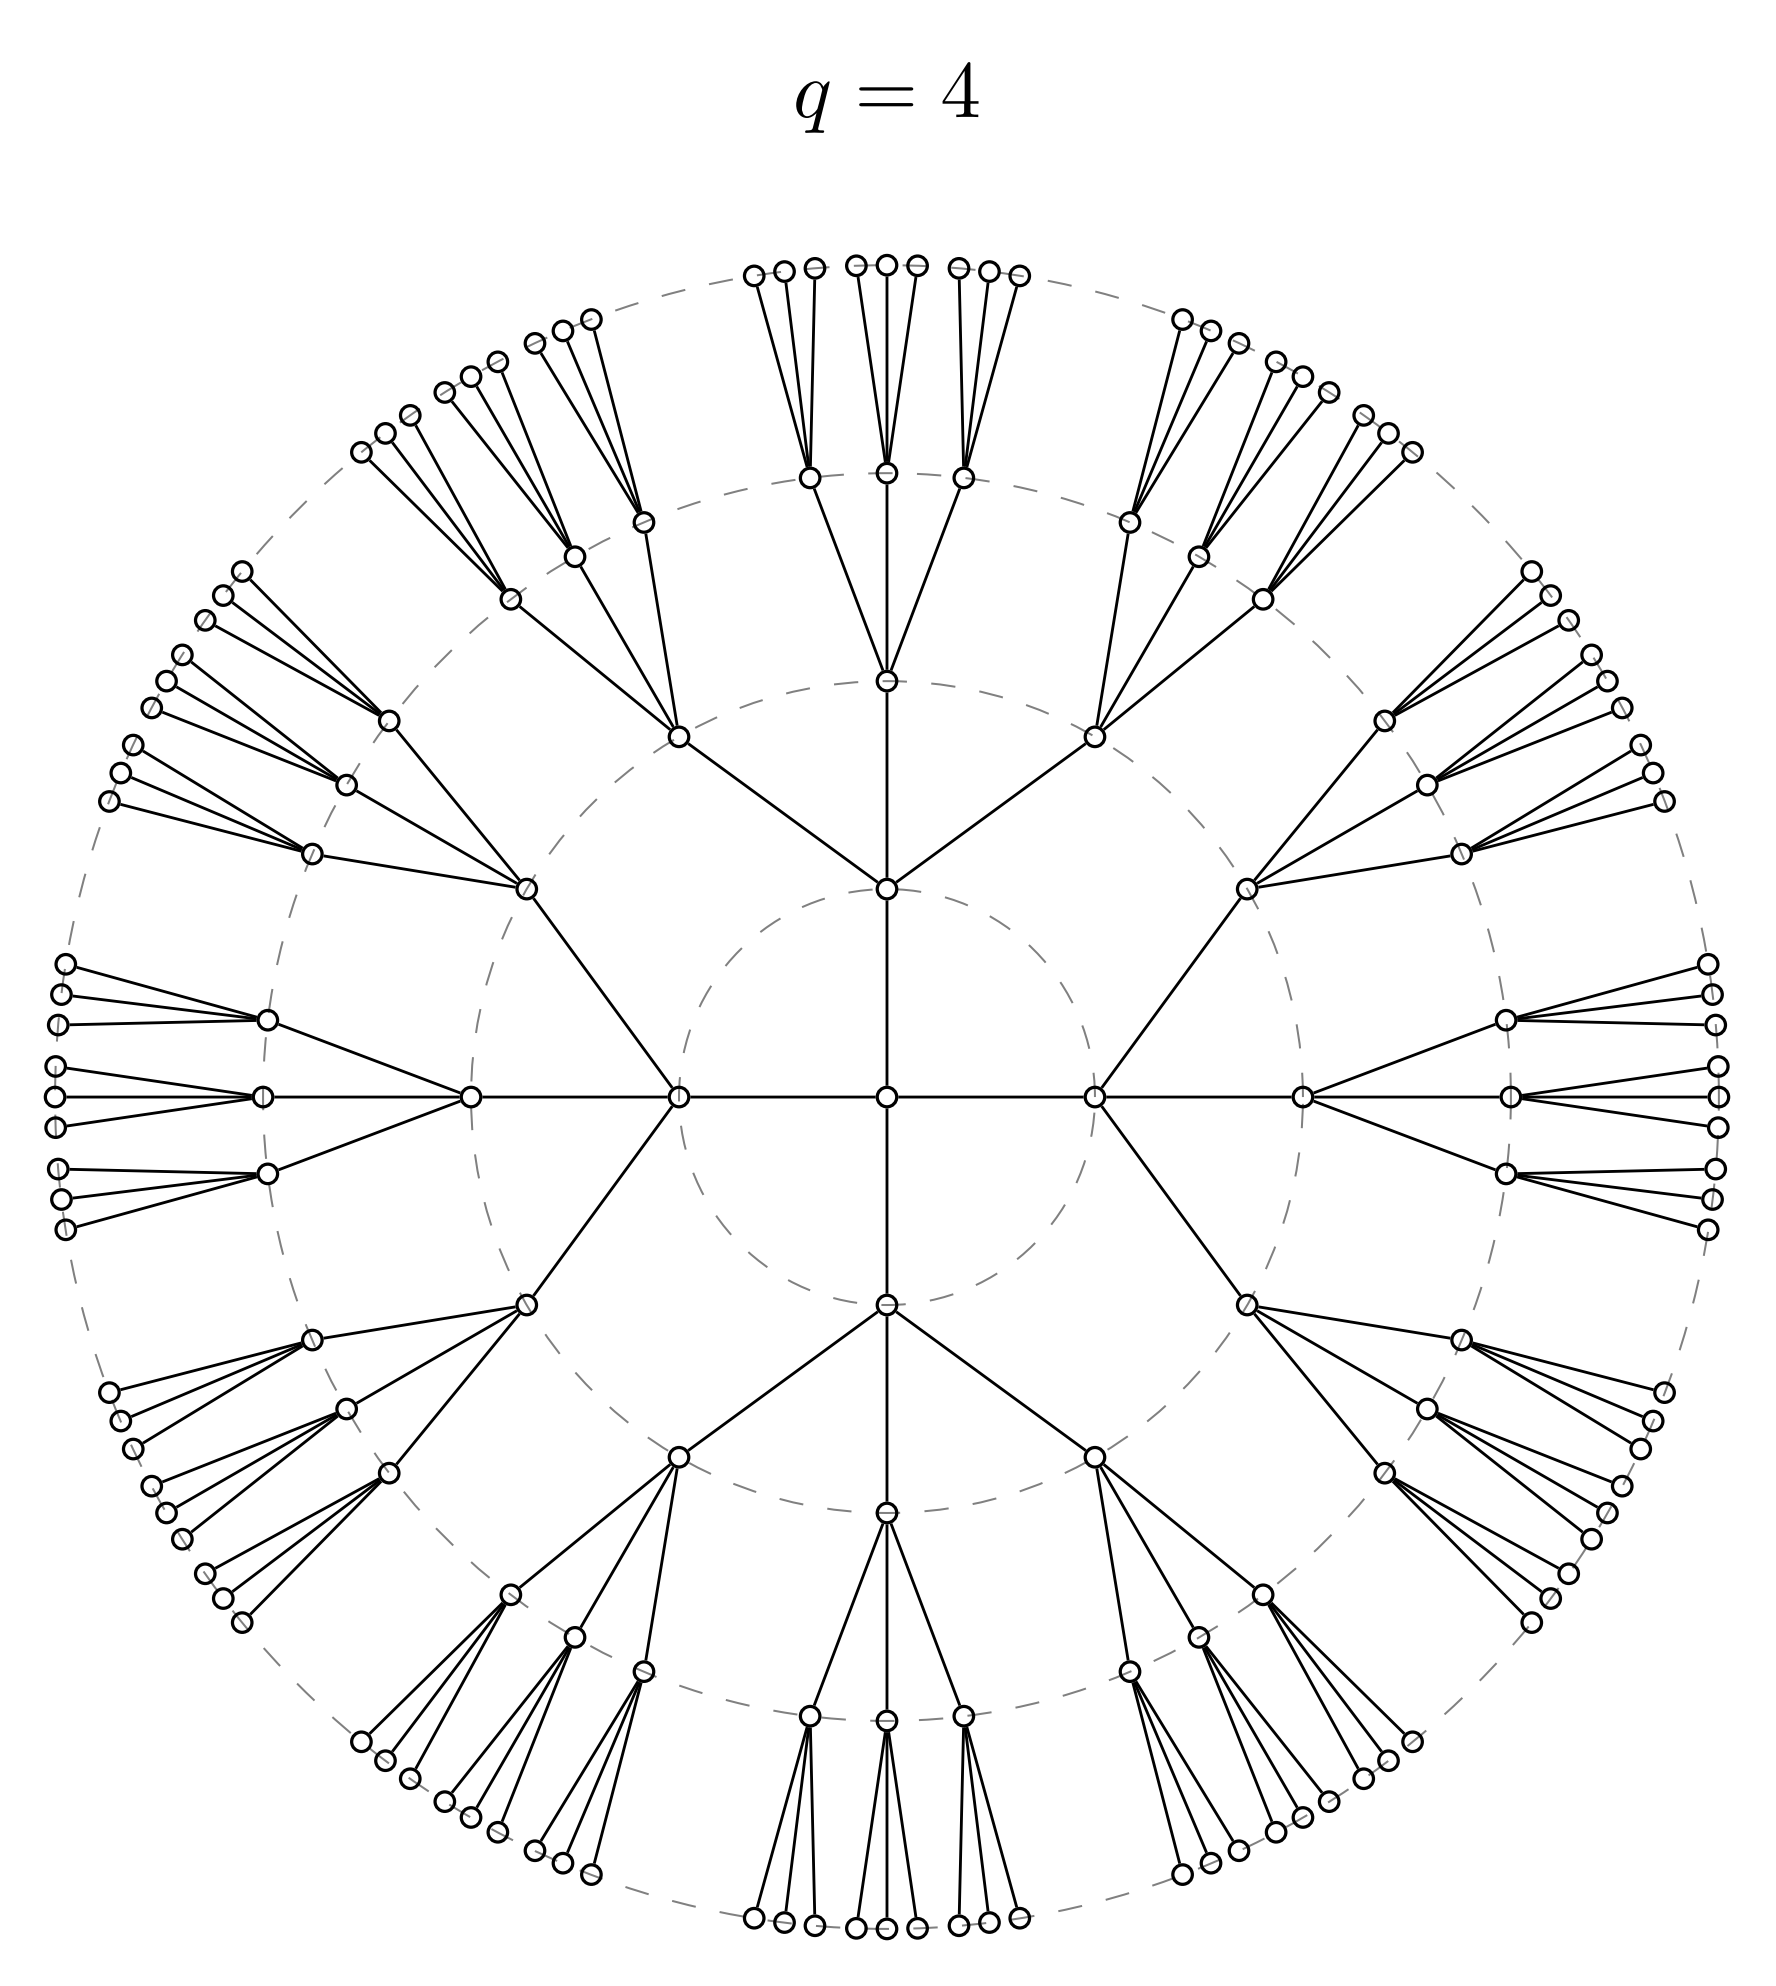
\includegraphics[width=\textwidth]{ising_model_fig/bethe_infinite_tree_level_3.png}
	\end{subfigure}
	\hfill
	\begin{subfigure}[b]{0.23\textwidth}
		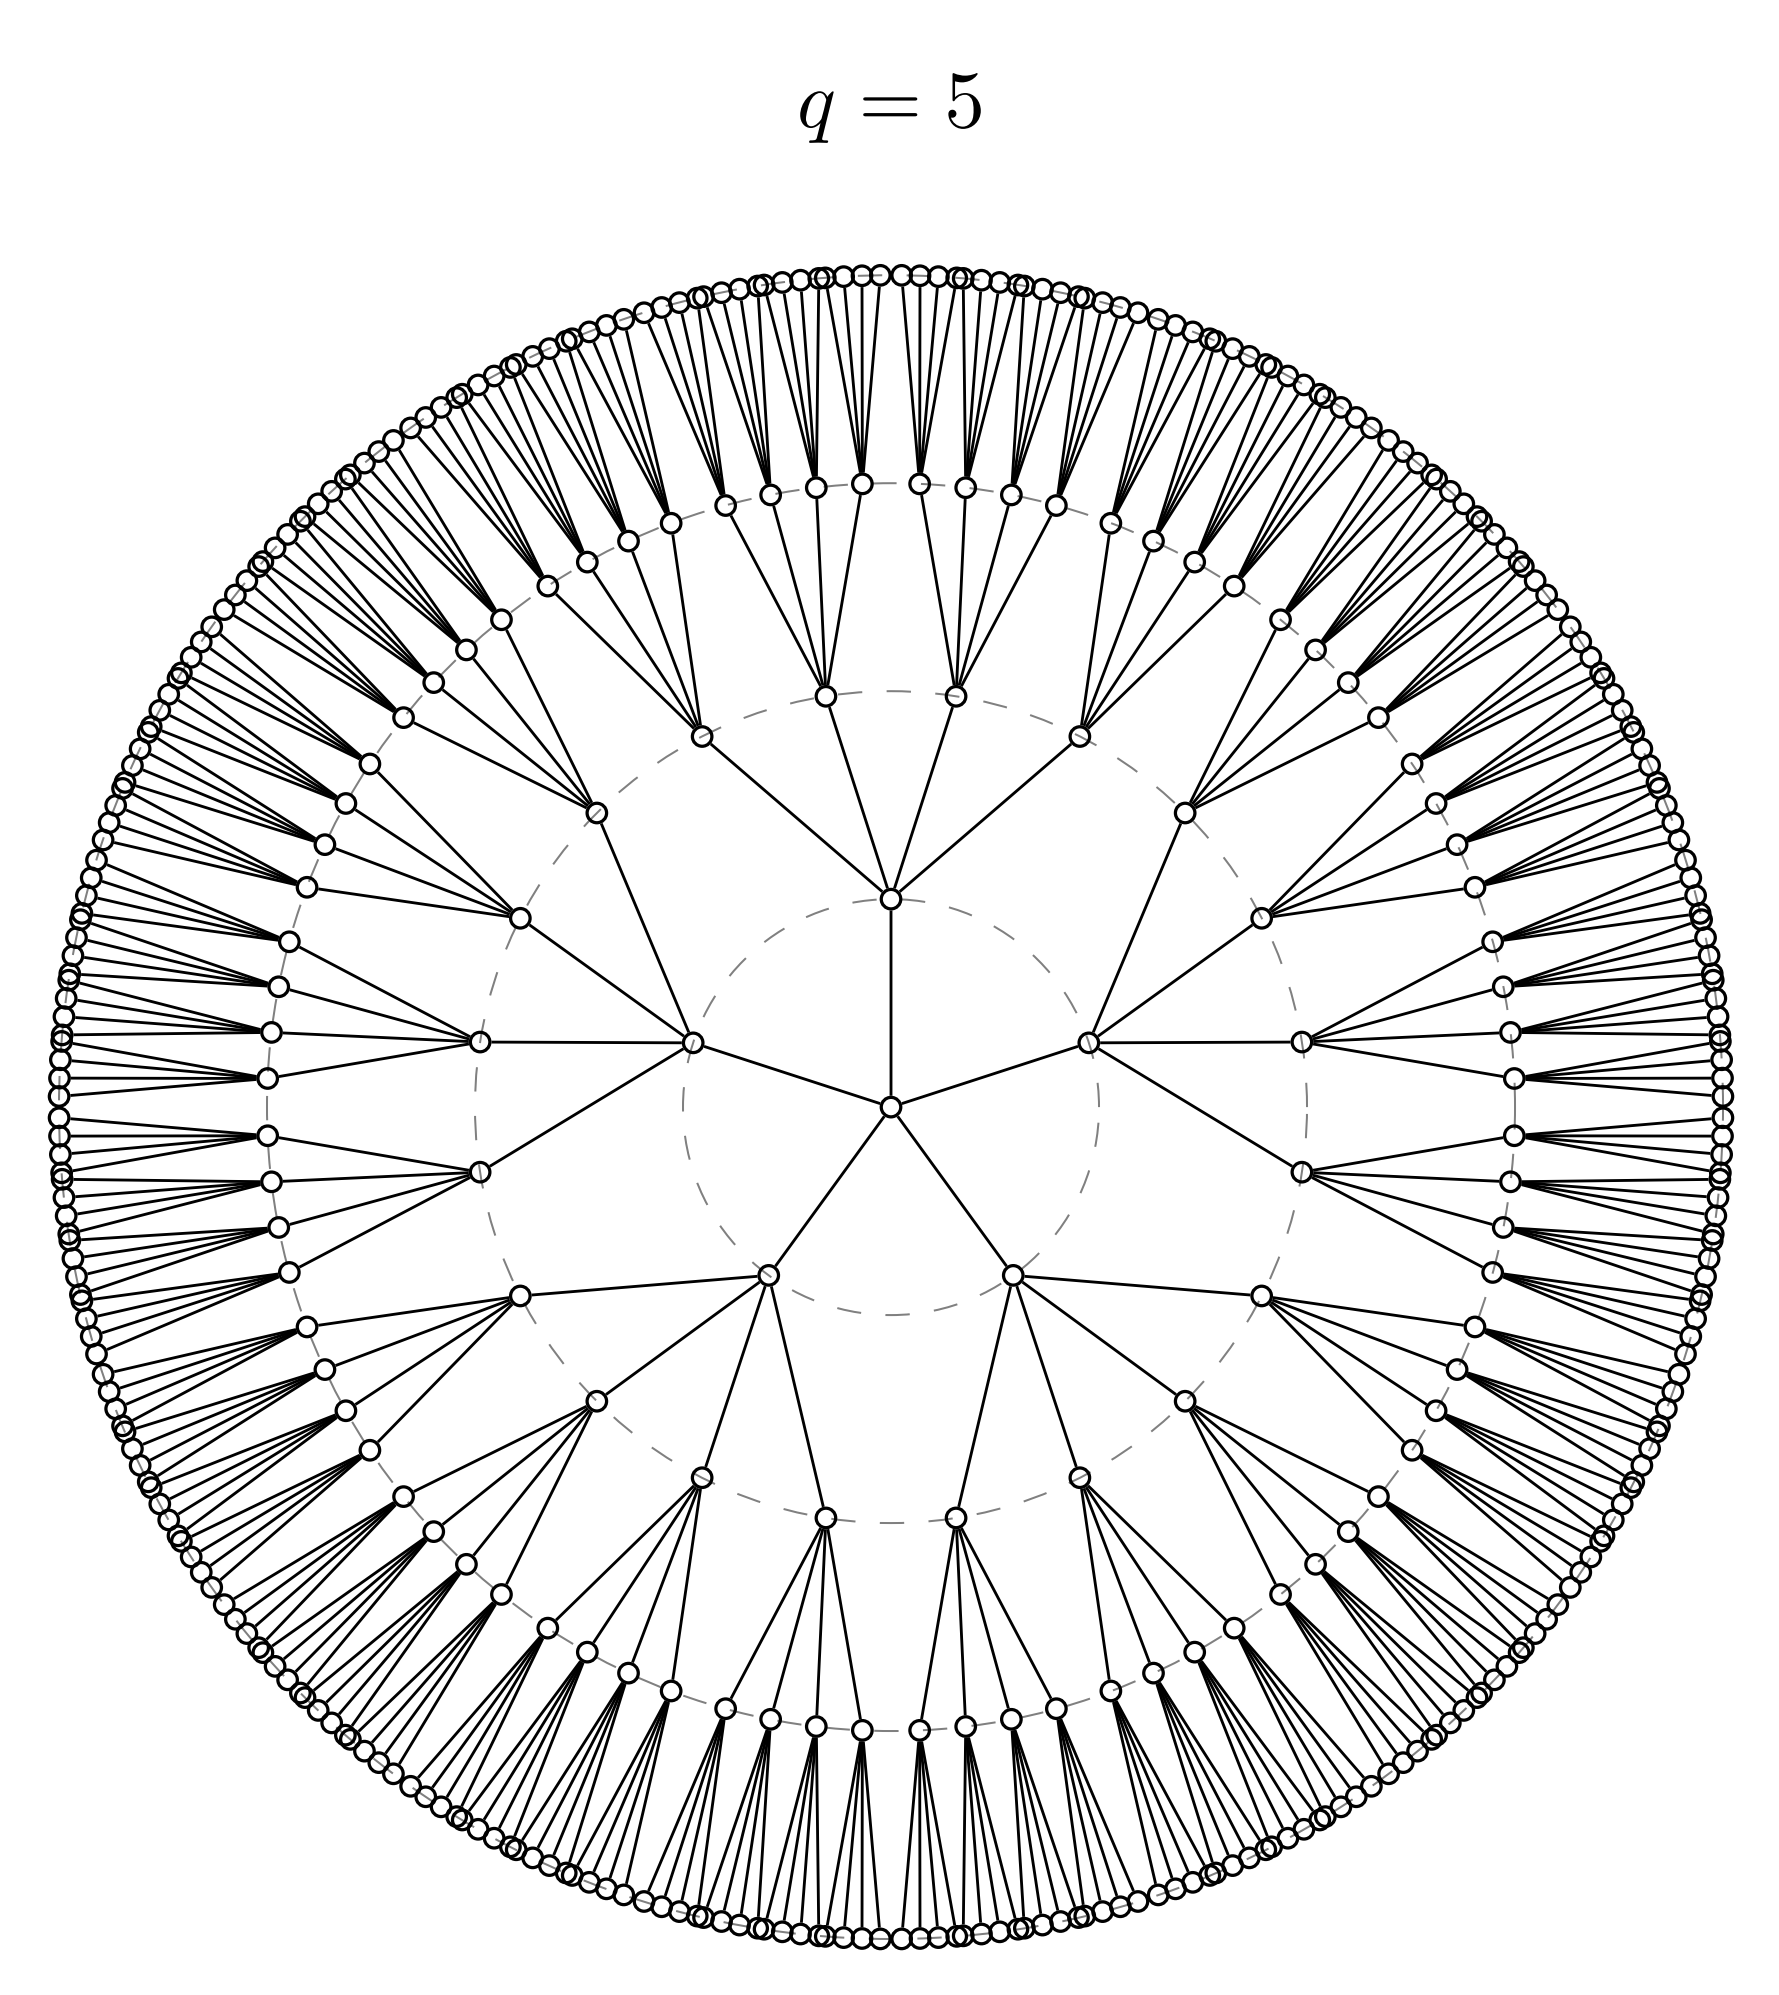
\includegraphics[width=\textwidth]{ising_model_fig/bethe_infinite_tree_level_4.png}
	\end{subfigure}
	\caption{Bethe无穷树示意图}
	\label{Bethe无穷树示意图}
\end{figure}
在Bethe晶格中，每个格点的配位数为\(d_i = q\)，总格点数\(N \to \infty\)（无穷大正则图），局部具有树的结构.由于相互作用定义上无向，故邻近对无向.在该条件下
\begin{equation*}
	\frac{S}{Nk} = -\frac{q}{2}\sum_{\vb{\sigma},\vb{\sigma}'}p_{\vb{\sigma}\vb{\sigma}'}\ln p_{\vb{\sigma}\vb{\sigma}'} + (q - 1)\sum_{\vb{\sigma}}p_{\vb{\sigma}}\ln p_{\vb{\sigma}}
\end{equation*}
其中
\begin{equation*}
	\sum_{\vb{\sigma},\vb{\sigma}'}p_{\vb{\sigma}\vb{\sigma}'} = \sum_{\vb{\sigma}}p_{\vb{\sigma}} = 1, \quad
	p_{\vb{\sigma}\vb{\sigma}'} = p_{\vb{\sigma}'\vb{\sigma}},\quad
	\sum_{\vb{\sigma}'}p_{\vb{\sigma}\vb{\sigma}'} = p_{\vb{\sigma}}
\end{equation*}

对于最简单的伊辛模型，每个格点只有磁矩朝上或朝下两个状态 \((\vb{\sigma} = \pm1)\)，记朝上的概率为 \(p_+\)、朝下的概率为 \(p_-\)；对于两个临近磁矩，记两者均为上的概率为 \(p_{++}\)、两者均为下的概率为 \(p_{--}\)、两者一上一下的概率为 \(p_{+-} = p_{-+}\).易知，各量满足
\begin{equation*}
	&p_+ + p_- = 1, \quad
	p_{++} + p_{--} + 2p_{+-} = 1, \\
	&p_{++} = (1 + p_+ - p_- - 2p_{+-})/2, \quad
	p_{--} = (1 - p_+ + p_- - 2p_{+-})/2
\end{equation*}

只考虑相邻自旋的相互作用，强度用\(J\)表征，则在外磁场\(B\)的作用下，体系哈密顿量为
\begin{equation*}
	\mathcal{H}_N = -\frac{1}{2}qNJ\left(p_{++} + p_{--} - p_{+-} - p_{-+}\right) - N\mu B\left(p_+ - p_-\right)
\end{equation*}

能量、熵为
\begin{equation*}
	\frac{E}{N} &= -\frac{qJ}{2}\left(p_{++} + p_{--} - 2p_{+-}\right) - \mu B\left(p_+ - p_-\right)\\
	\frac{S}{Nk} &= -\frac{q}{2}\sum_{\vb{\sigma},\vb{\sigma}'}p_{\vb{\sigma}\vb{\sigma}'}\ln p_{\vb{\sigma}\vb{\sigma}'} + (q - 1)\sum_{\vb{\sigma}}p_{\vb{\sigma}}\ln p_{\vb{\sigma}} \\
	&= -\frac{q}{2}\left(p_{++}\ln p_{++} + p_{--}\ln p_{--} + 2p_{+-}\ln p_{+-}\right) + (q - 1)\left(p_+\ln p_+ + p_-\ln p_-\right)
\end{equation*}

方便起见，先引入特征温度\(T_c\) 和约化温度\(t\)，后文将证明 \(T_c\) 恰为体系的临界温度
\begin{equation*}
	T_c = \frac{2J}{k}\left(\ln\frac{q}{q-2}\right)^{-1}, \quad
	t = \frac{T - T_c}{T_c}
\end{equation*}

代入无量纲化的外场和磁化序参量
\begin{equation*}
	h = \mu B/kT_c, \quad m = p_+ - p_-
\end{equation*}

得到自由能为
\begin{equation*}
	\Phi = \frac{F}{NkT_c} &=(1 + t)\Bigg[ \frac{q}{2}\Bigg(\frac{1 + m - 2p_{+-}}{2}\ln\frac{1 + m - 2p_{+-}}{2} + \frac{1 - m - 2p_{+-}}{2}\ln\frac{1 - m - 2p_{+-}}{2} + 2p_{+-}\ln p_{+-}\Bigg) \\
		&\quad- (q - 1)\Bigg(\frac{1 + m}{2}\ln\frac{1 + m}{2} + \frac{1 - m}{2}\ln\frac{1 - m}{2}\Bigg)\Bigg] -\frac{q}{4}\ln\frac{q}{q-2}\left(1 - 4p_{+-}\right) - hm
\end{equation*}

可见 \(\Phi = \Phi\left(m, t, p_{+-}, h\right)\).在稳态
\begin{equation*}
	\frac{\partial\Phi}{\partial p_{+-}} = 0, \quad \frac{\partial\Phi}{\partial m} = 0
\end{equation*}
解得
\begin{equation*}
	p_{+-} = \frac{1 - m^2}{2\left(1 + \sqrt{m^2 + (1 - m^2)\left(\frac{q}{q - 2}\right)^{\frac{2}{1 + t}}}\right)} ,\quad
	h = \frac{1 + t}{2}\left( \frac{q}{2}\ln\frac{1 + m - 2p_{+-}}{1 - m - 2p_{+-}} - (q - 1)\ln\frac{1 + m}{1 - m} \right)
\end{equation*}

引入参数\(a, \gamma\)，使得
\begin{equation*}
	\gamma = \frac{J}{kT} = \frac{1}{2(1 + t)}\ln\frac{q}{q - 2}, \quad
	m = \frac{\sinh(2a)}{\cosh(2a) + e^{-2\gamma}}
\end{equation*}

进而各量可化简为
\begin{equation*}
	p_{+-} &= \frac{e^{-2\gamma}}{2\left(\cosh(2a) + e^{-2\gamma}\right)}, \quad
	h = (t + 1)\left(a - \frac{q-1}{2}\ln\frac{\cosh(a + \gamma)}{\cosh(a - \gamma)}\right)\\
	p_{++} &= \frac{e^{2a}}{2\left(\cosh(2a) + e^{-2\gamma}\right)}, \quad
	p_{--} = \frac{e^{-2a}}{2\left(\cosh(2a) + e^{-2\gamma}\right)},\quad
	p_{\pm} = \frac{e^{-2\gamma} + e^{\pm 2a}}{2\left(\cosh(2a) + e^{-2\gamma}\right)}\\
	\chi &= \left(\frac{\partial m}{\partial h}\right)_t = \frac{4\left(1 + e^{-2\gamma}\cosh(2a)\right)\left(\cosh(2a) + e^{-2\gamma}\right)^{-2}}{(1 + t)\left[2 - (q - 1)\left(\tanh(a + \gamma) - \tanh(a - \gamma)\right)\right]}
\end{equation*}

临界温度附近，序参量很小，关于\(m\)展开得
\begin{equation*}
	a &= \frac{1 + e^{-2\gamma}}{2} m + \mathcal{O}\left(m^3\right), \\
	h &= \frac{(1 + t)\left(1 + e^{-2\gamma}\right)}{2}\left(1 - (q - 1)\tanh\gamma\right)m + \mathcal{O}\left(m^3\right)
\end{equation*}

根据定义，在临界点附近磁化率发散，因此临界点对应
\begin{equation*}
	(q - 1)\tanh\gamma = 1 \quad\implies\quad t = 0
\end{equation*}
这说明 \(T = T_c\) 就是临界温度

不难给出，在临界温度上
\begin{equation*}
	m\big|_{t = 0} = \left(\frac{3 q^2}{(q - 1) (q - 2)}\right)^{1/3} h^{1/3}
\end{equation*}

当外磁场为零(\(h=0\))时，\(a\)满足隐式关系
\begin{equation*}
	\left.\left(a - \frac{q-1}{2} \ln\frac{\cosh(a+\gamma)}{\cosh(a-\gamma)}\right)\right|_{h=0} = 0
\end{equation*}

能量、热容为
\begin{equation*}
	&\left.\frac{E}{N k T_c}\right|_{h=0} = -\frac{q}{4}  \frac{\cosh(2a) - e^{-2\gamma}}{\cosh(2a) + e^{-2\gamma}}\ln\frac{q}{q-2} \\
	&\left.\frac{C}{N k}\right|_{h=0} = \left.\frac{1}{N k} \frac{\d E}{\d T}\right|_{h=0} = \left.-\frac{1}{2} \left(\frac{T_c}{T}\right)^2 \ln\frac{q}{q-2} \frac{\d}{\d \gamma} \frac{E}{N k T_c}\right|_{h=0} \\
	&\quad = \left(\frac{T_c}{T}\right)^2 \frac{q e^{-2\gamma}}{2\left(\cosh(2a) + e^{-2\gamma}\right)^2} \left(\ln\frac{q}{q-2}\right)^2 \left[\cosh(2a) + \frac{(q-1)\sinh^2(2a)}{\cosh(2a) + \cosh(2\gamma) - (q-1)\sinh(2\gamma)}\right]
\end{equation*}

临界点附近
\begin{equation*}
	&m\big|_{h = 0} =
	\begin{cases}
		0,                                                                                & t \gtrsim 0,  \\
		\pm\sqrt{\displaystyle\frac{3}{2}\frac{q^2}{q - 1}\ln\frac{q}{q - 2}} (-t)^{1/2}, & t \lesssim 0.
	\end{cases}\qquad
	\chi\big|_{h = 0} =
	\begin{cases}
		\displaystyle\left(\frac{1}{2}(q - 2)\ln\frac{q}{q - 2}\right)^{-1} t^{-1}, & t \gtrsim 0,  \\
		\displaystyle\left((q - 2)\ln\frac{q}{q - 2}\right)^{-1} (-t)^{-1},         & t \lesssim 0.
	\end{cases}\\
	&\frac{E}{NkT_c}\bigg|_{h = 0} =
	\begin{cases}
		\displaystyle-\frac{1}{4}\frac{q}{q - 1}\ln\frac{q}{q - 2} + t\frac{q^2(q - 2)}{8(q - 1)^2}\left(\ln\frac{q}{q - 2}\right)^2, & t \gtrsim 0, \\[8pt]        \displaystyle-\frac{1}{4}\frac{q}{q - 1}\ln\frac{q}{q - 2} + t\frac{q^2(q - 2)(3q - 2)}{8(q - 1)^2}\left(\ln\frac{q}{q - 2}\right)^2, & t \lesssim 0.
	\end{cases}\\
	&\frac{C}{Nk}\bigg|_{h = 0} = \frac{1}{NkT_c}\frac{\d E}{\d t}\bigg|_{h = 0} =
	\begin{cases}
		\displaystyle\frac{q^2(q - 2)}{8(q - 1)^2}\left(\ln\frac{q}{q - 2}\right)^2,         & t \gtrsim 0,  \\[8pt]
		\displaystyle\frac{q^2(q - 2)(3q - 2)}{8(q - 1)^2}\left(\ln\frac{q}{q - 2}\right)^2, & t \lesssim 0.
	\end{cases}
\end{equation*}

\subsubsection{自由能展开解法}

将自由能在 \(t \to 0, m \to 0\) 处展开
\begin{equation*}
	\Phi &= -mh
	+ \left( -\ln 2 + \frac{q}{4}\ln\frac{q(q - 2)}{(q - 1)^2} \right)
	+ \left[ -\ln 2 + \frac{q}{4(q - 1)}\Bigl( (q - 2)\ln(q - 2) - 2(q - 1)\ln(q - 1) + q\ln q \Bigr) \right] t \\
	&\quad\quad- \frac{q^2(q - 2)}{16(q - 1)^2} \left( \ln\frac{q}{q - 2} \right)^2 t^2
	+ \frac{q - 2}{4} \ln\frac{q}{q - 2} \, t m^2
	+ \frac{(q - 2)(q - 1)}{12q^2} m^4 + \mathcal{O}\left( t^3, t^2 m^2, t m^4 \right).
\end{equation*}

可以写成
\begin{equation*}
	\Phi &= -hm + \left(a_0 + a_1 t + a_2 t^2\right) + b_1 t m^2 + c_0 m^4 + \mathcal{O}\left(t^3, t^2m^2, tm^4\right)\\
	a_2 &= -\frac{q^2(q - 2)}{16(q - 1)^2}\left(\ln\frac{q}{q - 2}\right)^2, \quad b_1 = \frac{q - 2}{4}\ln\frac{q}{q - 2}, \quad c_0 = \frac{(q - 2)(q - 1)}{12q^2}
\end{equation*}

根据朗道相变理论，在临界点附近的稳态
\begin{equation*}
	\frac{\partial\Phi}{\partial m} = 0 \quad\implies\quad h = 2 b_1 t m + 4 c_0 m^3
\end{equation*}

进而可以得到各热力学量在临界点附近的幂次行为 (要求 \(a_2 < 0, b_1 > 0, c_0 > 0\))
\begin{equation*}
	&m\big|_{t = 0} = \left(\frac{1}{4 c_0}\right)^{1/3} h^{1/3},\quad
	m\big|_{h = 0} =
	\begin{cases}
		0,                                                & t \gtrsim 0, \\
		\displaystyle\sqrt{\frac{b_1}{2 c_0}} (-t)^{1/2}, & t \lesssim 0
	\end{cases}\\
	&\chi\big|_{h = 0} = \left(\frac{\partial m}{\partial h}\right)_t\bigg|_{h = 0} =
	\begin{cases}
		\displaystyle\frac{1}{2 b_1} t^{-1},    & t \gtrsim 0,  \\[8pt]
		\displaystyle\frac{1}{4 b_1} (-t)^{-1}, & t \lesssim 0.
	\end{cases}\\
	&\frac{C}{Nk}\bigg|_{h = 0} = -\frac{\d^2\Phi(t, m(t))}{\d t^2}\bigg|_{h = 0} =
	\begin{cases}
		-2 a_2,                                    & t \gtrsim 0,  \\
		\displaystyle-2 a_2 + \frac{b_1^2}{2 c_0}, & t \lesssim 0.
	\end{cases}
\end{equation*}

不难验证，朗道的理论和对严格解取临界点极限给出了相同的结果

特别地，\(q = 2\) 的一维伊辛链显然是无环树，因此 Bethe 方法给出的结果是严格的.重新记
\begin{equation*}
	\tilde{h} = h/(1 + t) = \mu B/kT, \quad \tilde{\chi} = \chi (1 + t), \quad \ln\frac{q}{q - 2} = 2 \gamma (1 + t)
\end{equation*}
根据如上讨论得
\begin{equation*}
	a &= \frac{1}{2}\,\mathrm{arcsinh}\left(e^{2 \gamma} \sinh\tilde{h} \left(\cosh\tilde{h} + \sqrt{e^{-4 \gamma} + \sinh^2\tilde{h}}\right)\right) \\
	m &= \frac{\sinh\tilde{h}}{\sqrt{e^{-4 \gamma} + \sinh^2\tilde{h}}}, \quad
	\tilde{\chi} = \frac{\cosh\tilde{h} \, e^{-4 \gamma}}{\left(e^{-4 \gamma} + \sinh^2\tilde{h}\right)^{3/2}}, \quad
	p_{\pm} = \frac{1}{2}\left(1 \pm \frac{\sinh\tilde{h}}{\sqrt{e^{-4 \gamma} + \sinh^2\tilde{h}}}\right) \\
	p_{++} &= \frac{1}{2}\frac{e^{\tilde{h}} \left(\sqrt{e^{-4 \gamma} + \sinh^2\tilde{h}} + \sinh\tilde{h}\right)}{\sqrt{e^{-4 \gamma} + \sinh^2\tilde{h}} \left(\cosh\tilde{h} + \sqrt{e^{-4 \gamma} + \sinh^2\tilde{h}}\right)} \\
	p_{--} &= \frac{1}{2}\frac{e^{-\tilde{h}} \left(\sqrt{e^{-4 \gamma} + \sinh^2\tilde{h}} - \sinh\tilde{h}\right)}{\sqrt{e^{-4 \gamma} + \sinh^2\tilde{h}} \left(\cosh\tilde{h} + \sqrt{e^{-4 \gamma} + \sinh^2\tilde{h}}\right)} \\
	p_{+-} &= \frac{1}{2}\frac{e^{-4 \gamma}}{\sqrt{e^{-4 \gamma} + \sinh^2\tilde{h}} \left(\cosh\tilde{h} + \sqrt{e^{-4 \gamma} + \sinh^2\tilde{h}}\right)}\\
	\frac{E}{NJ} &= \frac{\sqrt{e^{-4\gamma} + \sinh^2\tilde{h}} \left( -\cosh\tilde{h} + \sqrt{e^{-4\gamma} + \sinh^2\tilde{h}} \right)}{\sqrt{e^{-4\gamma} + \sinh^2\tilde{h}} \left( \cosh\tilde{h} + \sqrt{e^{-4\gamma} + \sinh^2\tilde{h}} \right)}
\end{equation*}

由所得精确解可见，在零外场下磁化强度始终为零，从而一维伊辛模型不存在有限温度相变

\subsubsection{平均场解法}
在 Bethe 晶格上，去掉中心节点后，其相邻节点之间不再通过其它路径相连，因此在给定中心自旋的条件下这些邻居统计独立.在这一特殊结构下，Bethe 方法与平均场方法给出等价的结果.

具体而言，将中心状态\(\vb{\sigma}_0\)和它周围的\(q\)个状态\(\vb{\sigma}_1\cdots\vb{\sigma}_q\)视为一个集团，集团外边节点的影响用有效场 \(B'\) 代替，有效场作用于\(\vb{\sigma}_1\cdots\vb{\sigma}_q\)上，则集团的哈密顿量为
\begin{equation*}
	\mathcal{H}_q = -J \vb{\sigma}_0 \sum_{i=1}^q \vb{\sigma}_i - \mu B \vb{\sigma}_0 - \mu (B + B') \sum_{i=1}^q \vb{\sigma}_i
\end{equation*}

记
\begin{equation*}
	\tilde{h} = \beta\mu B, \quad \tilde{h}' = \beta\mu B', \quad \gamma = \beta J
\end{equation*}

则配分函数为
\begin{equation*}
	Q = \sum_{\vb{\sigma}_0, \{\vb{\sigma}_i\}} \exp\left[\tilde{h} \vb{\sigma}_0 + \left(\tilde{h} + \tilde{h}' + \gamma \vb{\sigma}_0\right) \sum_{i=1}^q \vb{\sigma}_i\right] = Q_+ + Q_-
\end{equation*}
式中 \(Q_{\pm}\) 对应 \(\vb{\sigma}_0 = \pm1\)，即
\begin{equation*}
	Q_{\pm} = \sum_{\{\vb{\sigma}_i\}} \exp\left[\pm\tilde{h} + \left(\tilde{h} + \tilde{h}' \pm \gamma\right) \sum_{i=1}^q \vb{\sigma}_i\right] = e^{\pm\tilde{h}} \prod_{i=1}^q \sum_{\vb{\sigma}_i=\pm1} \exp\left[\left(\tilde{h} + \tilde{h}' \pm \gamma\right) \vb{\sigma}_i\right] = e^{\pm\tilde{h}} \left(2\cosh\left(\tilde{h} + \tilde{h}' \pm \gamma\right)\right)^q
\end{equation*}

中心状态平均值、近邻状态平均值为
\begin{equation*}
	\langle \vb{\sigma}_0 \rangle = \frac{Q_+ - Q_-}{Q_+ + Q_-}, \quad \langle \vb{\sigma}_i \rangle = \frac{1}{q}\frac{\partial\ln Q}{\partial \tilde{h}'} = \frac{Q_+ \tanh\left(\tilde{h} + \tilde{h}' + \gamma\right) + Q_- \tanh\left(\tilde{h} + \tilde{h}' - \gamma\right)}{Q_+ + Q_-}
\end{equation*}

系统是平移不变的，因此 \(\langle \vb{\sigma}_0 \rangle = \langle \vb{\sigma}_i \rangle\)，得到
\begin{equation*}
	e^{2 \tilde{h}'} = \left(\frac{\cosh\left(\tilde{h} + \tilde{h}' + \gamma\right)}{\cosh\left(\tilde{h} + \tilde{h}' - \gamma\right)}\right)^{q - 1}
\end{equation*}

记 \(a = \tilde{h} + \tilde{h}'\)，得
\begin{equation*}
	\tilde{h} = a - \frac{q - 1}{2}\ln\frac{\cosh(a + \gamma)}{\cosh(a - \gamma)}
\end{equation*}

进而状态为\(\pm1\)的概率为
\begin{equation*}
	p_{\pm} = \frac{Q_{\pm}}{Q} = \frac{e^{-2 \gamma} + e^{\pm2 a}}{2\left(\cosh(2a) + e^{-2 \gamma}\right)}
\end{equation*}

磁化强度序参量为
\begin{equation*}
	m = p_+ - p_- = \frac{\sinh(2a)}{\cosh(2a) + e^{-2 \gamma}}
\end{equation*}

对于相邻状态的组合，将配分函数写为
\begin{equation*}
	Q = \sum_{\vb{\sigma}_0, \vb{\sigma}_1} \left(2\cosh\left(\tilde{h} + \tilde{h}' + \gamma \vb{\sigma}_0\right)\right)^{q - 1} \exp\left[\tilde{h} \vb{\sigma}_0 + \left(\tilde{h} + \tilde{h}' + \gamma \vb{\sigma}_0\right) \vb{\sigma}_1\right] = Q_{++} + Q_{--} + Q_{+-} + Q_{-+}
\end{equation*}
式中 \(Q_{\pm\pm}\) 对应 \(\vb{\sigma}_0 = \pm1, \vb{\sigma}_1 = \pm1\)，代入平移不变性条件，即
\begin{equation*}
	Q_{++} &= e^{2a - \tilde{h}' + \gamma} \left(2\cosh\left(\tilde{h} + \tilde{h}' + \gamma\right)\right)^{q - 1}, \quad Q_{--} = e^{-2a - \tilde{h}' + \gamma} \left(2\cosh\left(\tilde{h} + \tilde{h}' + \gamma\right)\right)^{q - 1}\\
	Q_{+-} &= Q_{-+} = e^{-\tilde{h}' - \gamma} \left(2\cosh\left(\tilde{h} + \tilde{h}' + \gamma\right)\right)^{q - 1}
\end{equation*}

因此
\begin{equation*}
	p_{++} &= \frac{Q_{++}}{Q} = \frac{e^{2a}}{2\left(\cosh(2a) + e^{-2 \gamma}\right)}, \quad p_{--} = \frac{Q_{--}}{Q} = \frac{e^{-2a}}{2\left(\cosh(2a) + e^{-2 \gamma}\right)}\\
	p_{+-} &= p_{-+} = \frac{Q_{+-}}{Q} = \frac{e^{-2 \gamma}}{2\left(\cosh(2a) + e^{-2 \gamma}\right)}
\end{equation*}

再根据体系哈密顿量
\begin{equation*}
	\mathcal{H}_N = -\frac{1}{2}qNJ\left(p_{++} + p_{--} - p_{+-} - p_{-+}\right) - N\mu B\left(p_+ - p_-\right)
\end{equation*}

可以得到与之前完全一致的结论.

\subsection{Bragg-Williams近似}


Bragg-Williams(B-W)近似忽略最近邻关联，把成对概率因子分解为单点概率的乘积 (\(p_{\sigma\sigma'} = p_{\sigma} p_{\sigma'}\))，因此只在格点数、配位数为同阶无穷大时 (比如完全图 \(K_{N}\), \(N \to \infty\)) 严格成立.其严格性虽远不及Bethe方法，但形式更为简洁，且临界指数一致，在此补充介绍.B-W近似给出但格点的能量、熵为
\begin{align*}
	\frac{E}{N}  & = -\frac{1}{2} qJ \left(p_{++} + p_{--} - p_{+-} - p_{-+}\right) - \mu B \left(p_{+} - p_{-}\right)                \\
	             & = -\frac{1}{2} qJ \left(p_{+} - p_{-}\right)^2 - \mu B \left(p_{+} - p_{-}\right) = -\frac{1}{2} qJ m^2 - \mu B m. \\
	\frac{S}{Nk} & = -\sum_{\sigma} p_{\sigma} \ln p_{\sigma} = -\frac{1+m}{2} \ln\frac{1+m}{2} - \frac{1-m}{2} \ln\frac{1-m}{2}.
\end{align*}

方便起见，先引入特征温度\(T_c\)、约化温度\(t\)、无量纲化外场\(h\)，后文将证明 \(T_c\) 恰为体系的临界温度
\begin{equation*}
	T_c = \frac{qJ}{k}, \quad t = \frac{T - T_c}{T_c}, \quad h = \frac{\mu B}{k T_c}.
\end{equation*}

则自由能可以写作
\begin{align*}
	\Phi & = \frac{F}{NkT_c} = -\frac{1}{2} m^2 - hm + (1+t) \left[\frac{1+m}{2} \ln\frac{1+m}{2} + \frac{1-m}{2} \ln\frac{1-m}{2}\right].
\end{align*}

在稳态 \(\partial\Phi/\partial m = 0\)，解得
\begin{equation*}
	m = \tanh\left(\frac{m + h}{1 + t}\right), \quad \chi = \left(\frac{\partial m}{\partial h}\right)_t = \frac{1 - m^2}{t + m^2}.
\end{equation*}

临界温度附近，序参量很小，关于\(m\)展开得
\begin{equation*}
	h = t m + \mathcal{O}(m^3).
\end{equation*}

根据定义，在临界点附近，磁化率发散，这说明 \(t = 0\) 恰是临界温度.不难给出，在临界温度上
\begin{equation*}
	\left.m\right|_{t=0} = 3^{1/3} h^{1/3}.
\end{equation*}

当外磁场为零 (\(h = 0\)) 时，各量化简为
\begin{equation*}
	\left(m - \tanh\frac{m}{1+t}\right)_{h=0} = 0, \quad
	\left.\frac{E}{NkT_c}\right|_{h=0} = -\frac{1}{2} m^2, \quad
	\left.\frac{C}{Nk}\right|_{h=0} = \left.\frac{1}{Nk} \frac{\d E}{\d T}\right|_{h=0} = \frac{m^2 (1 - m^2)}{(1+t)(m^2 + t)}.
\end{equation*}

临界点附近
\begin{equation*}
	\left.m\right|_{h=0} &=
	\begin{cases}
		0,                      & t \gtrsim 0,  \\
		\pm\sqrt{3} (-t)^{1/2}, & t \lesssim 0.
	\end{cases}
	\qquad
	\left.\chi\right|_{h=0} =
	\begin{cases}
		t^{-1},                & t \gtrsim 0,  \\
		\frac{1}{2} (-t)^{-1}, & t \lesssim 0.
	\end{cases}\\
	\left.\frac{E}{NkT_C}\right|_{h=0} &=
	\begin{cases}
		0,              & t \gtrsim 0,  \\
		\dfrac{3}{2} t, & t \lesssim 0.
	\end{cases}
	\qquad
	\left.\frac{C}{Nk}\right|_{h=0} = \left.\frac{1}{NkT_C} \frac{\d E}{\d t}\right|_{h=0} =
	\begin{cases}
		0,            & t \gtrsim 0,  \\
		\dfrac{3}{2}, & t \lesssim 0.
	\end{cases}
\end{equation*}

可见，B-W近似给出与Bethe方法相同的临界指数，但系数有所差别.

同样，通过在临界点附近展开自由能
\begin{equation*}
	\left.\Phi\right|_{t \to 0, m \to 0} = -(1+t) \ln 2 - hm + \frac{1}{2} t m^2 + \frac{1}{12} m^4 + \mathcal{O}(t^3, t^2 m^2, t m^4) \Rightarrow a_2 = 0, \quad b_1 = \frac{1}{2}, \quad c_0 = \frac{1}{12}.
\end{equation*}
代入朗道相变理论，不难给出相同的结果；

平均场也将给出等价的自洽方程
\begin{equation*}
	P_{\sigma_0} \propto e^{\beta \sigma_0 (\mu B + q J m)} \quad\implies\quad m = \langle \sigma_0 \rangle = \sum_{\sigma_0} \sigma_0 P_{\sigma_0} = \tanh\left(\frac{m + h}{1 + t}\right)
\end{equation*}
式中
\begin{equation*}
	1 + t = \frac{T}{T_c} = \frac{kT}{qJ}, \quad h = \frac{\mu B}{k T_c}.
\end{equation*}
进而给出相同的结果.
\begin{figure}[htbp]
	\centering
	\begin{subfigure}[b]{0.49\textwidth}
		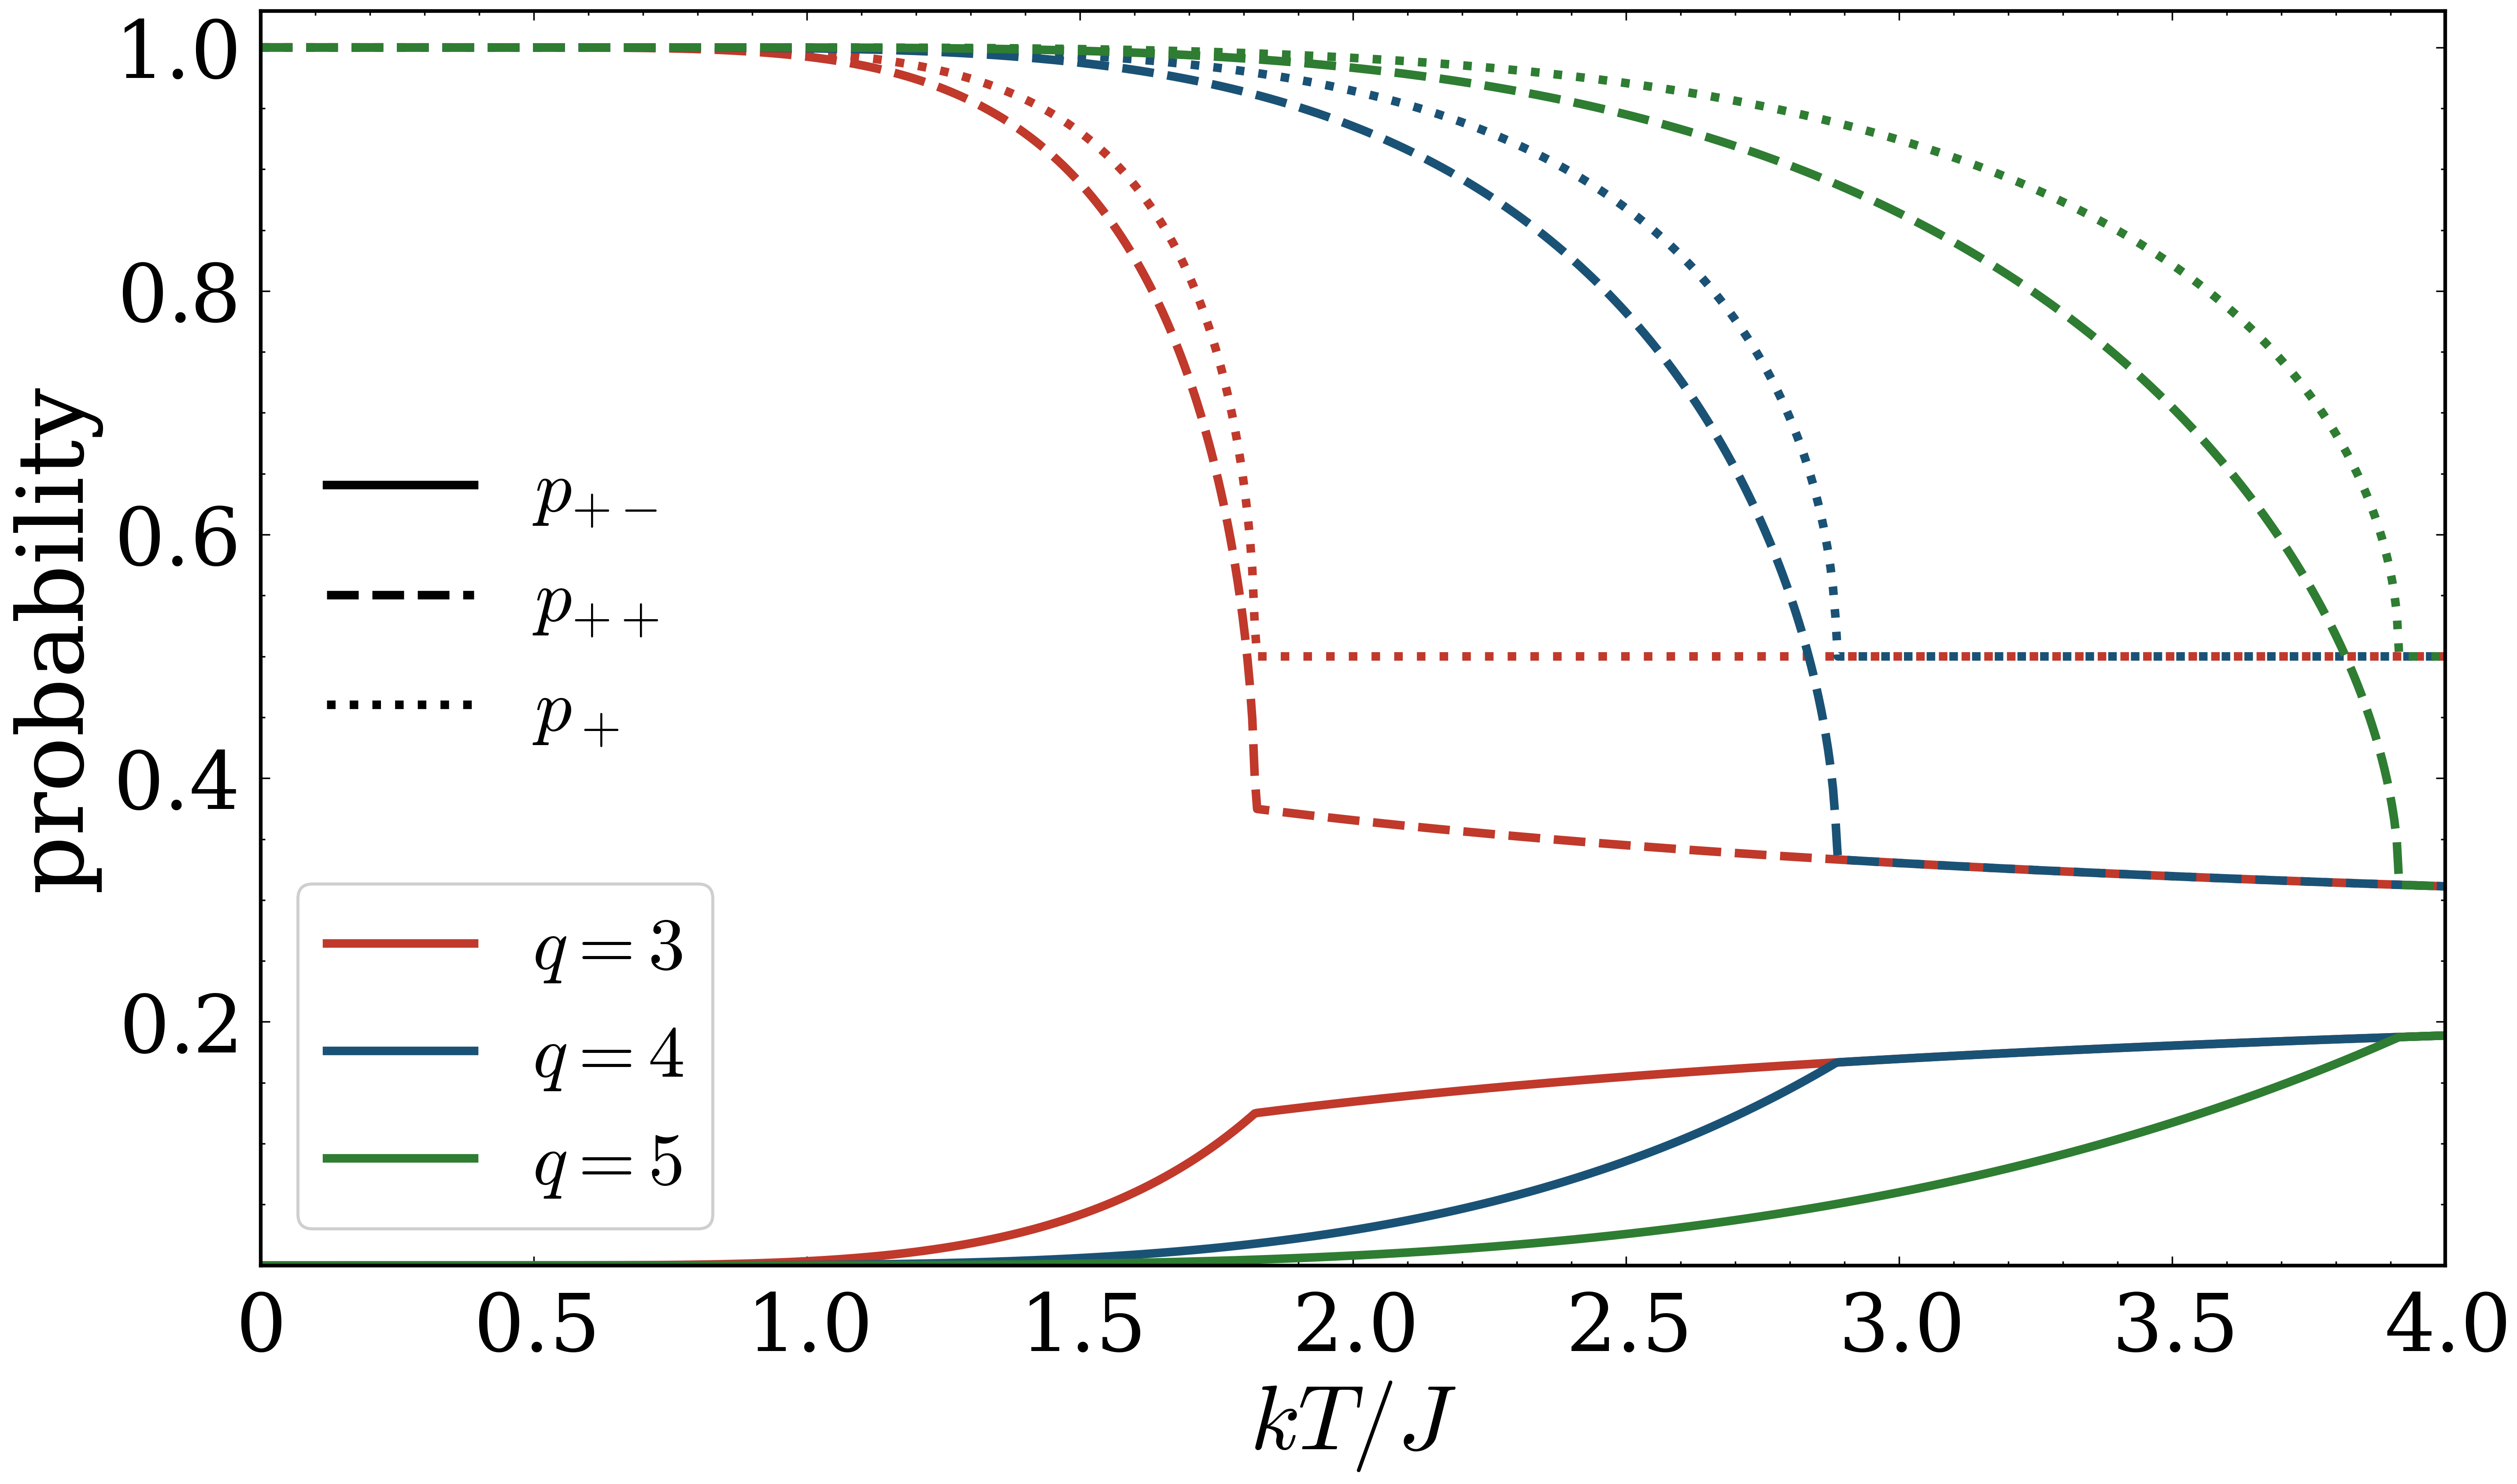
\includegraphics[width=\textwidth]{ising_model_fig/state_probability.png}
		\caption{状态概率}
		\label{各统计量随温度变化图-状态概率}
	\end{subfigure}
	\hfill
	\begin{subfigure}[b]{0.49\textwidth}
		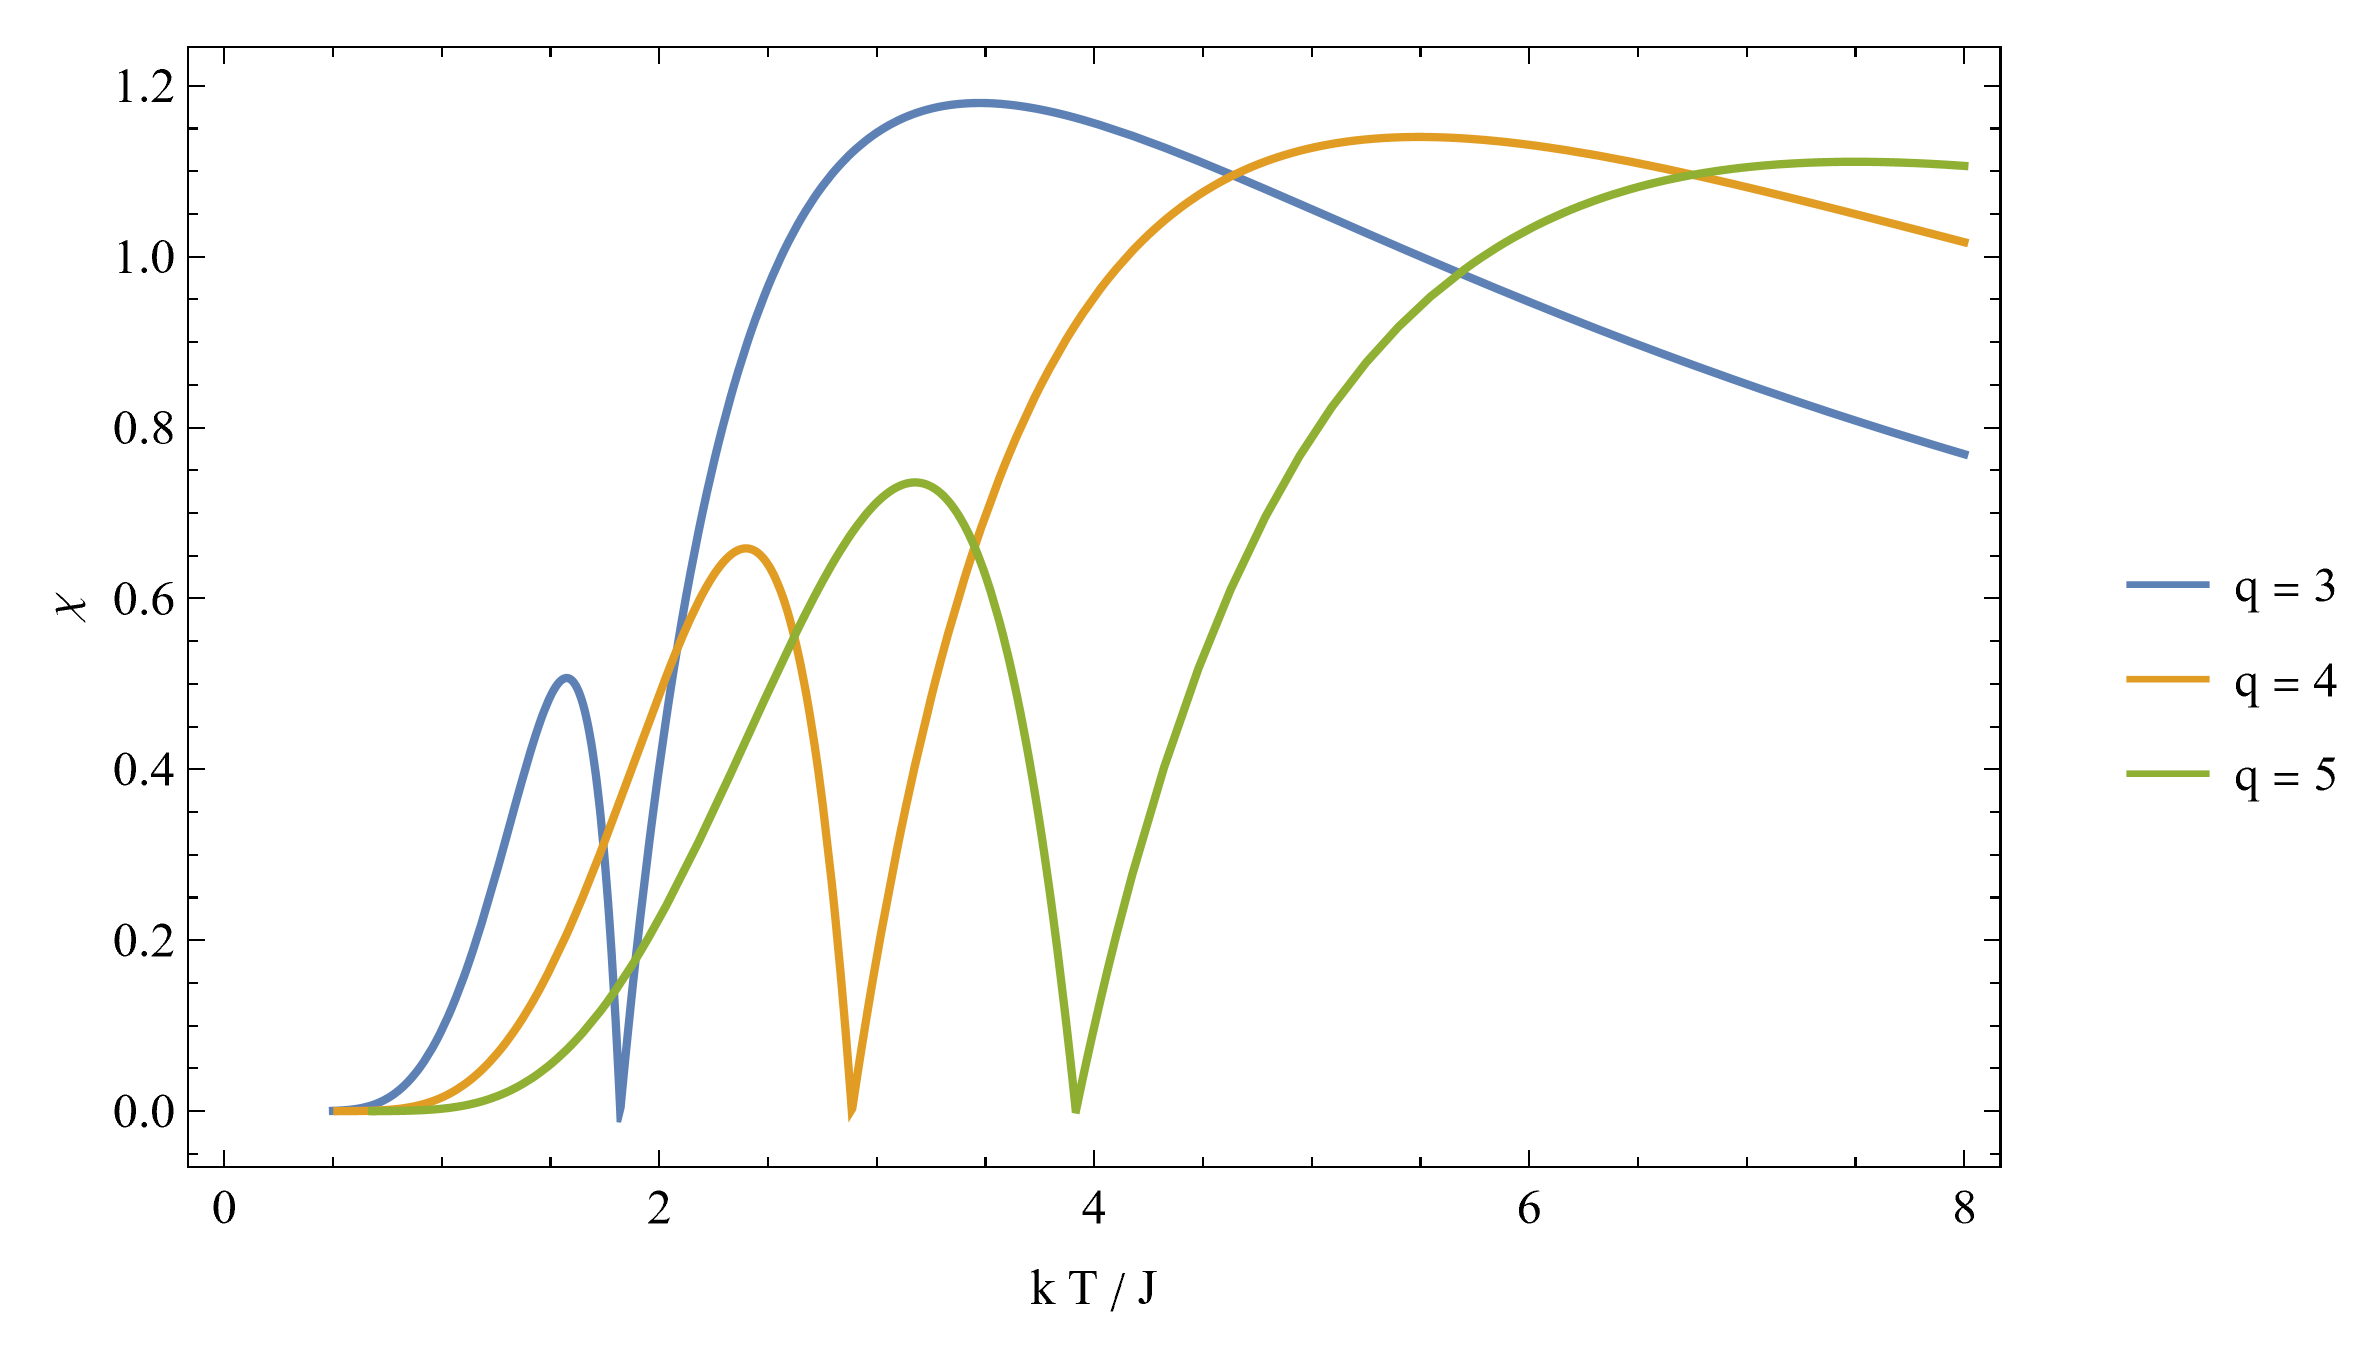
\includegraphics[width=\textwidth]{ising_model_fig/magnetic_susceptibility.png}
		\caption{磁化率}
		\label{各统计量随温度变化图-磁化率}
	\end{subfigure}

	\vspace{0.1cm}
	\begin{subfigure}[b]{0.49\textwidth}
		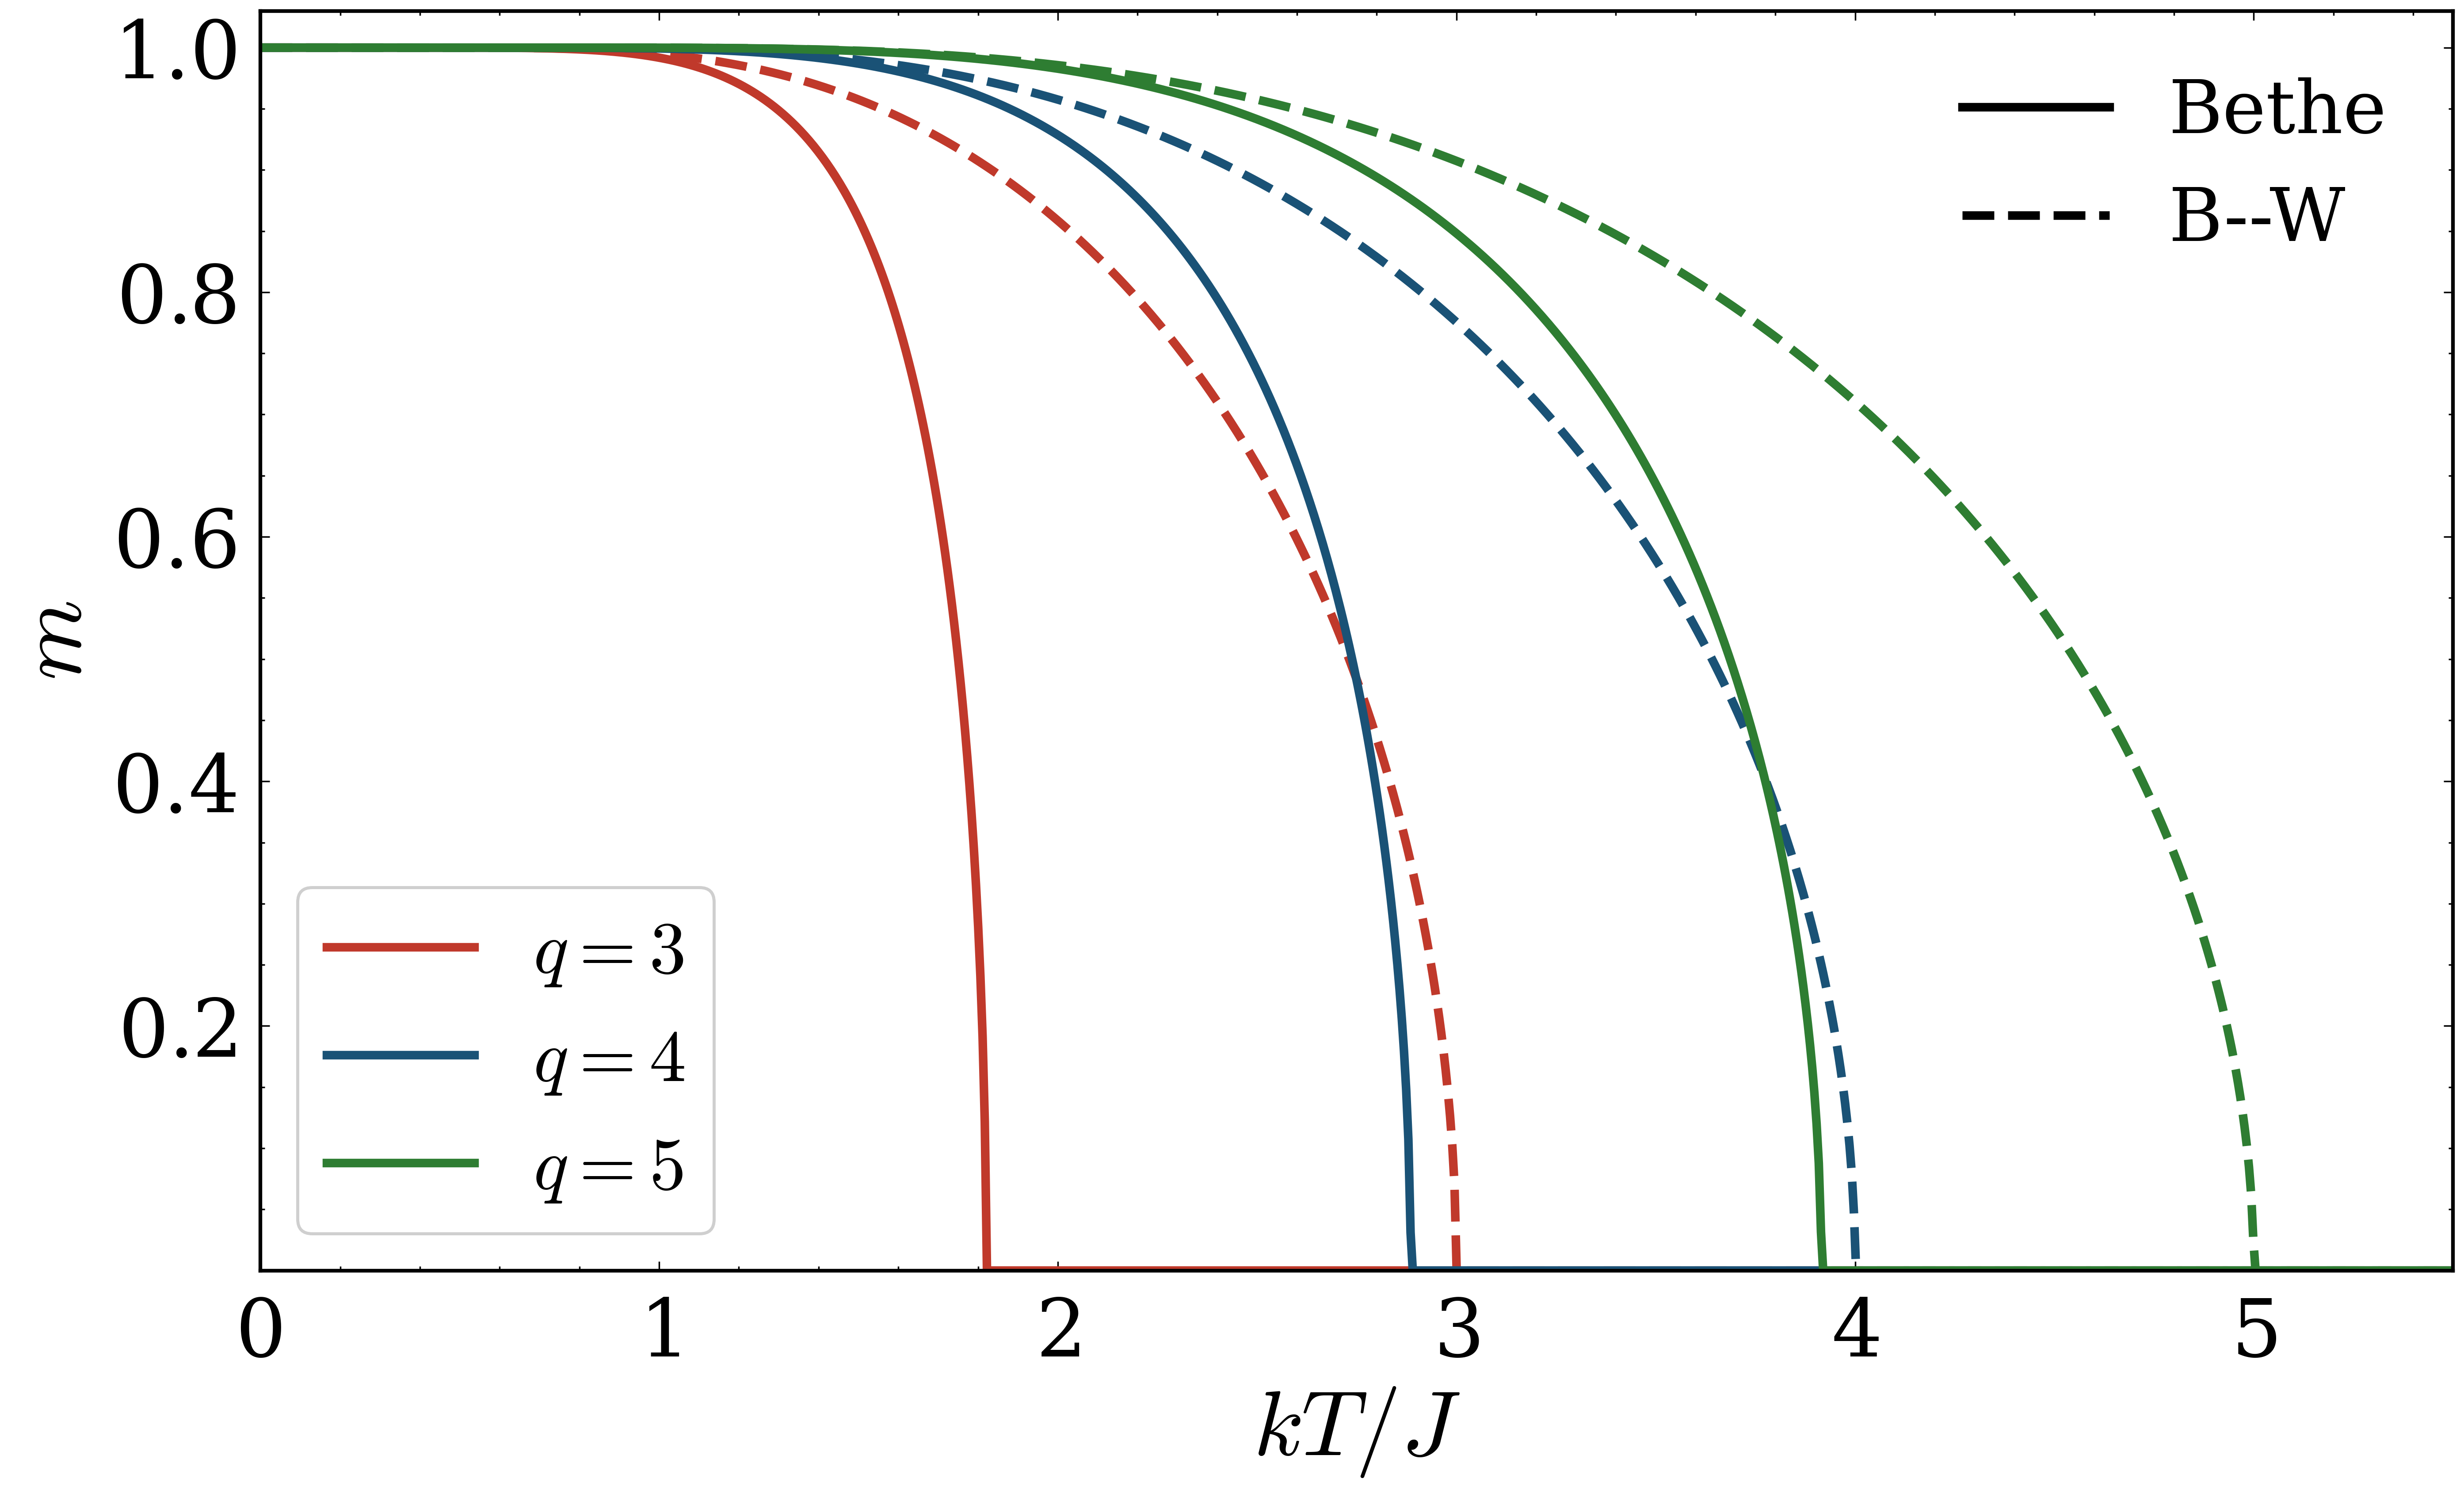
\includegraphics[width=\textwidth]{ising_model_fig/order_parameter.png}
		\caption{序参量}
		\label{各统计量随温度变化图-序参量}
	\end{subfigure}
	\hfill
	\begin{subfigure}[b]{0.49\textwidth}
		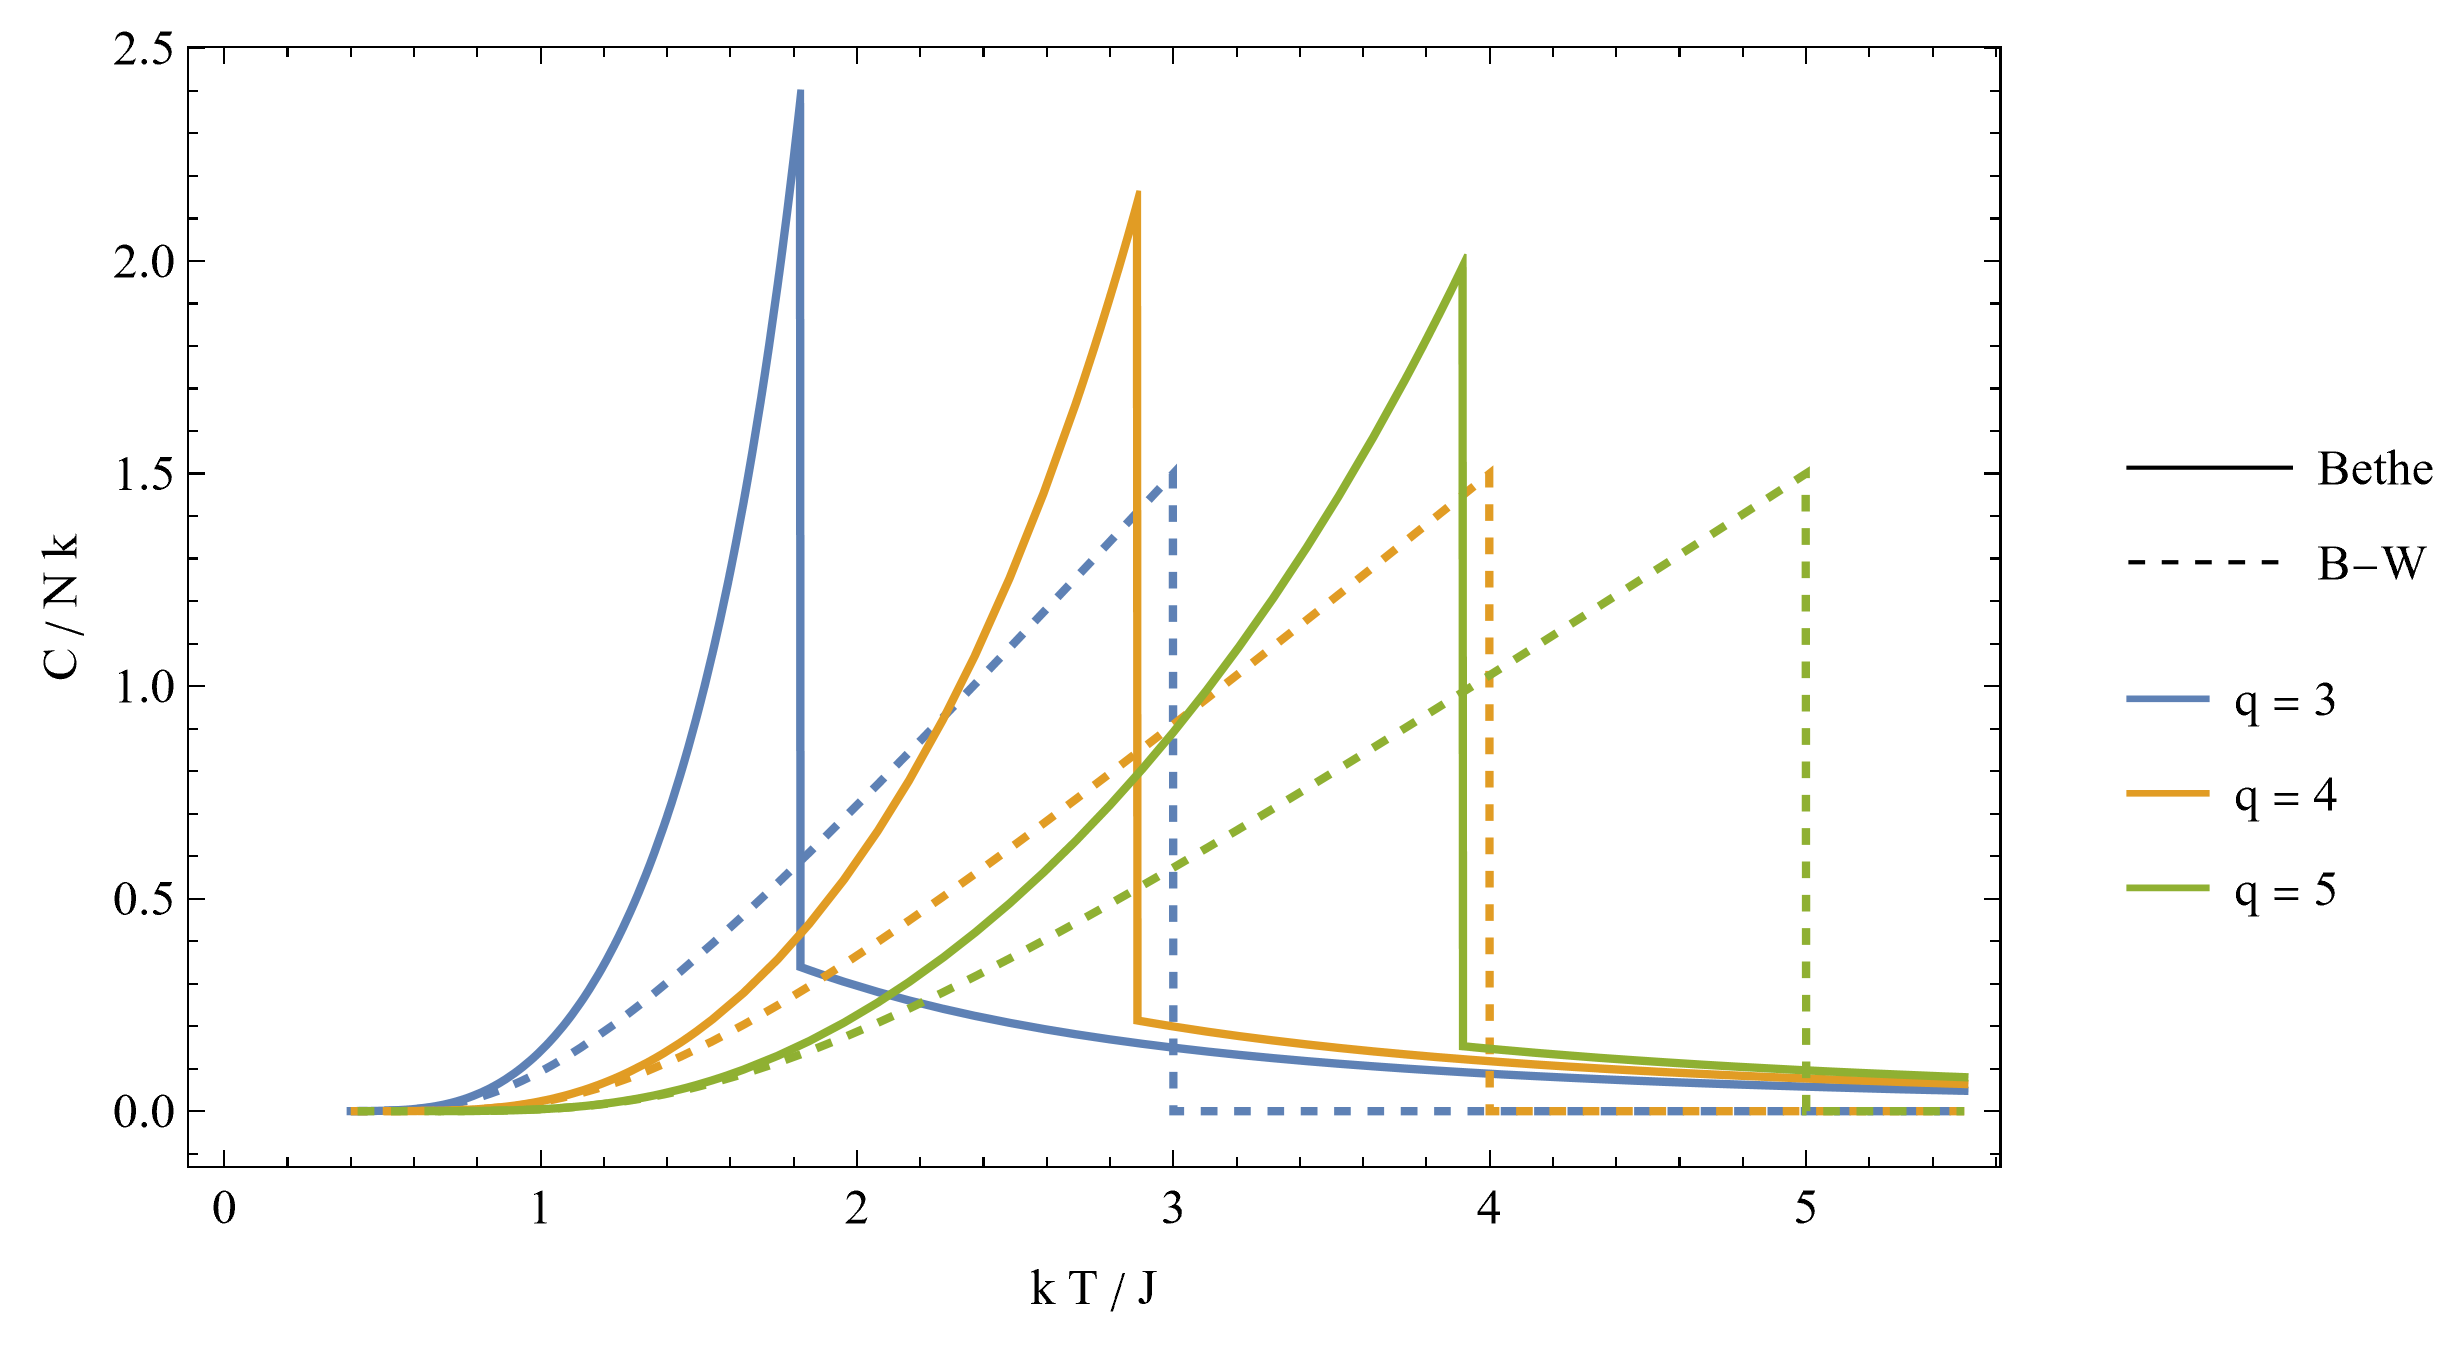
\includegraphics[width=\textwidth]{ising_model_fig/heat_capacity.png}
		\caption{热容}
		\label{各统计量随温度变化图-热容}
	\end{subfigure}
	\caption{各统计量随温度变化图}
	\label{各统计量随温度变化图}
\end{figure}

